\documentclass{beamer}

\usepackage[utf8]{inputenc}
\usepackage[english]{babel}

\usepackage{graphicx}
\usepackage{amsmath}
\usepackage{mathtools}
\usepackage{wrapfig}
\usepackage{amsfonts}
\usepackage{csquotes}
\usepackage{epigraph}
\usepackage{float}
\usepackage{lipsum}
\usepackage{blindtext}
\usepackage{multirow}
\usepackage[ruled,vlined]{algorithm2e}
\usepackage{bm}
\usepackage{xcolor}
\usepackage{upgreek}
\usepackage{calc}
\usepackage{lscape}
\usepackage[font={scriptsize}]{caption}
\usepackage{systeme}


% TYPESETTING SUGAR
\def\leq{\leqslant}
\def\geq{\geqslant}

\usetheme{Madrid}
\usecolortheme[rgb={0.0,0.4,0.5}]{structure}
%-----------------------------------------------%
%-----------------------------------------------%


%
% TITLE SLIDE
%

\makeatletter
\setbeamertemplate{footline}{%
  \leavevmode%
  \hbox{\begin{beamercolorbox}[wd=.4\paperwidth,ht=2.5ex,dp=1.125ex,leftskip=.20cm plus1fill,rightskip=.20cm, center]{author in head/foot}%
    \usebeamerfont{author in head/foot}\insertshortauthor%
  \end{beamercolorbox}%
  \begin{beamercolorbox}[wd=.6\paperwidth,ht=2.5ex,dp=1.125ex,leftskip=.20cm,rightskip=.20cm plus1fil, center]{title in head/foot}%
    \usebeamerfont{title in head/foot}\insertshorttitle \hspace*{2.5ex}
    \insertframenumber{}/\inserttotalframenumber
  \end{beamercolorbox}}%
  \vskip0pt%
}
\makeatother

\title[\textit{CoViD-19} daily positive-case count prediction for Northern India]{\textit{CoViD-19} daily positive-case count \\prediction for Northern India}

\author[E. Ballarin $|$ R. Corti $|$ A. Tasciotti]{Emanuele Ballarin \\ Roberto Corti \\ Arianna Tasciotti}
\institute[]{Department of Mathematics and Geosciences, University of Trieste}
\date[]{\textit{Statistical Methods for Data Science}\\ Final Project $\sim$ July 2020}

\titlegraphic{
\includegraphics[width=1.25cm,height=1.3cm,keepaspectratio]{dssclogo.png}
	\hspace*{93.04mm}~% Horizontal space is tailored for 1.3cm square logos
	
\includegraphics[width=1.3cm,height=1.25cm,keepaspectratio]{logouniv.png}
}

%-----------------------------------------------%
%-----------------------------------------------%



%
% ADAPTIVE TABLE OF CONTENTS
%

\AtBeginSection[]
{
	\begin{frame}
		\frametitle{\textit{We are here...}}
		\tableofcontents[currentsection]
	\end{frame}
}

%-----------------------------------------------%
%-----------------------------------------------%



%
% DOCUMENT
%

\begin{document}

% Insert title slide
\frame{\titlepage}

%-----------------------------------------------%

\section{\textit{Introductory Overview}}{

%% P.S. 01
\begin{frame}
\frametitle{\textit{CoViD-19} in India: What and Why}
\framesubtitle{A global pandemic hitting hard the World's most populous democracy}
\begin{itemize}
	\item{\textbf{CoViD-19}: clinical expression of the \textbf{human-host} infectious disease caused by \textit{SARS-CoV-2}. Probably resulted from \textit{animal spillover}.}
	\item{Identified during \textbf{Dec 2019}, in Wuhan (Hubei, China).\\As of Jul, 1, 2020: $> 10.4\ \text{mln}$ cases, $> 511\text{k}$ deaths worldwide.}
\end{itemize}
\hfill
\begin{itemize}
	\item{\textbf{India}:\\Outbreak: ongoing since January 2020;\\1st $\in$ Asia and 4th $\in$ World country w.r.t. number of confirmed cases.}
	\item{Further focus on \textbf{Northern India}, i.e. the $9$ regions of: \\
	\textit{Uttar Pradesh, Chandigarh, Haryana, Delhi, Himachal Pradesh, Jammu and Kashmir, Punjab, Rajasthan, Uttarakhand}.}
\end{itemize}
\end{frame}

%% P.S. 02
\begin{frame}
	\frametitle{Formal Problem Statement}
	\framesubtitle{Understanding aims and limits of present work}
		Predict the number of new \textbf{daily} confirmed cases of \textit{CoViD-19} for \textbf{Northern India}, on a \textit{per-state} basis.
		%\hfill
		\break
		\begin{itemize}
			\item{Up to \textbf{$\textbf{10}$ days} since the last known daily \textit{data-point};}
			\item{While also providing \textbf{predictive uncertainty} information;}
			\item{Trying to favor \textbf{parameter parsimony}, \textbf{theoretically-sound} methods, \textbf{explainability} and \textbf{interpretability} of the results;}
			\item{By using only publicly-available data from the Internet.}
		\end{itemize}
	\hfill

	\textit{Medical data $\rightarrow$ extra-care required!}
\end{frame}
}
\section{\textit{DataWorks}}{
%---------------------------------------------%
%% D.C. 01
\begin{frame}
	\frametitle{Data Gathering}
	\framesubtitle{Finding the source(s) of knowledge}
		\begin{itemize}
			\item{
				Kaggle (Sudalai Rajkumar):
				\begin{itemize}
					\item{Age grouping, early-outbreak ($<$ Mar 2020) [IMHW];}
					\item{Per-state/per-date individual counting data [IMHW];}
					\item{Confirmed individuals, early-outbreak [\textit{covid19india}, volunt.];}
					\item{Statewise geopolitical / hospital information [Indian Census 2011].}
				\end{itemize}
			}
		\hfill
		\item{
	\textit{covid19india}'s API:
	\begin{itemize}
		\item{Per-state/per-date individual counting data; additional [volunt.];}
		\item{Confirmed individuals, early-outbreak; additional [volunt.].}
	\end{itemize}
}
		\end{itemize}

	\hfill\break
	In a pipelined, incremental, \textbf{reproducible} manner (\textsf{bash}, \textsf{binutils}, \textsf{R}).

	\hfill\break

	Self-contained \textit{data arrangement}: \textbf{KF-CV} and \textbf{train/test} split.

\end{frame}

%% D.C. 02
\begin{frame}
	\frametitle{Data Cleaning}
	\framesubtitle{Making \textit{human world} more \textit{machine-friendly}}

	\textbf{Principled} drop of data:
	\begin{itemize}
		\item{Unnecessary data for the task considered (e.g. \textit{lat/long} of labs);}
		\item{Technical-only information (e.g. IDs, index keys);}
		\item{Non-easily-processable data (with \textit{permitted tools}; e.g. raw text).}
	\end{itemize}

	\hfill

	Removal of to-be-\textbf{duplicated} data:
	\begin{itemize}
		\item{To avoid \textit{by-design} duplication and variance inflation.\\ \textit{More on this in the forthcoming!}}
	\end{itemize}

	\hfill

	Dealing with \textsf{\textbf{NA}}s:
	\begin{itemize}
		\item{Simple removal ($\rightarrow$ upfront information loss);}
		\item{Data-carry-on ($\rightarrow$ information-theoretical justification for T.S.s).}
	\end{itemize}

\end{frame}

%---------------------------------------------%
%%Slide 1.3.1
\begin{frame}
	\frametitle{Data pre-processing}
	\framesubtitle{Making \textit{machine-friendly} more \textit{model-friendly}}

	Data transformations:
	\begin{itemize}
		\item Numerical encoding of categorical or string variables (e.g. date, sex);
		\item Daily averaging of patient information;
		\item Compressed, still informative quantities \\ (e.g. urban population, rural population $\rightarrow$ urbanization).
	\end{itemize}
	~\\
	Introduction of new variables:
	\begin{itemize}
		\item Daily metrics (e.g. daily positives, daily swabs);
		\item 3-, 4- lagged components (daily swabs), 10- lagged components (daily positive and average daily patient's age and sex).
	\end{itemize}

\end{frame}
%---------------------------------------------%
%---------------------------------------------%
%% SLIDE 1.4.1:
\begin{frame}
	\frametitle{Exploratory Data Analysis: Demographic features (1)}
	\framesubtitle{A country of contrasts}
	\center 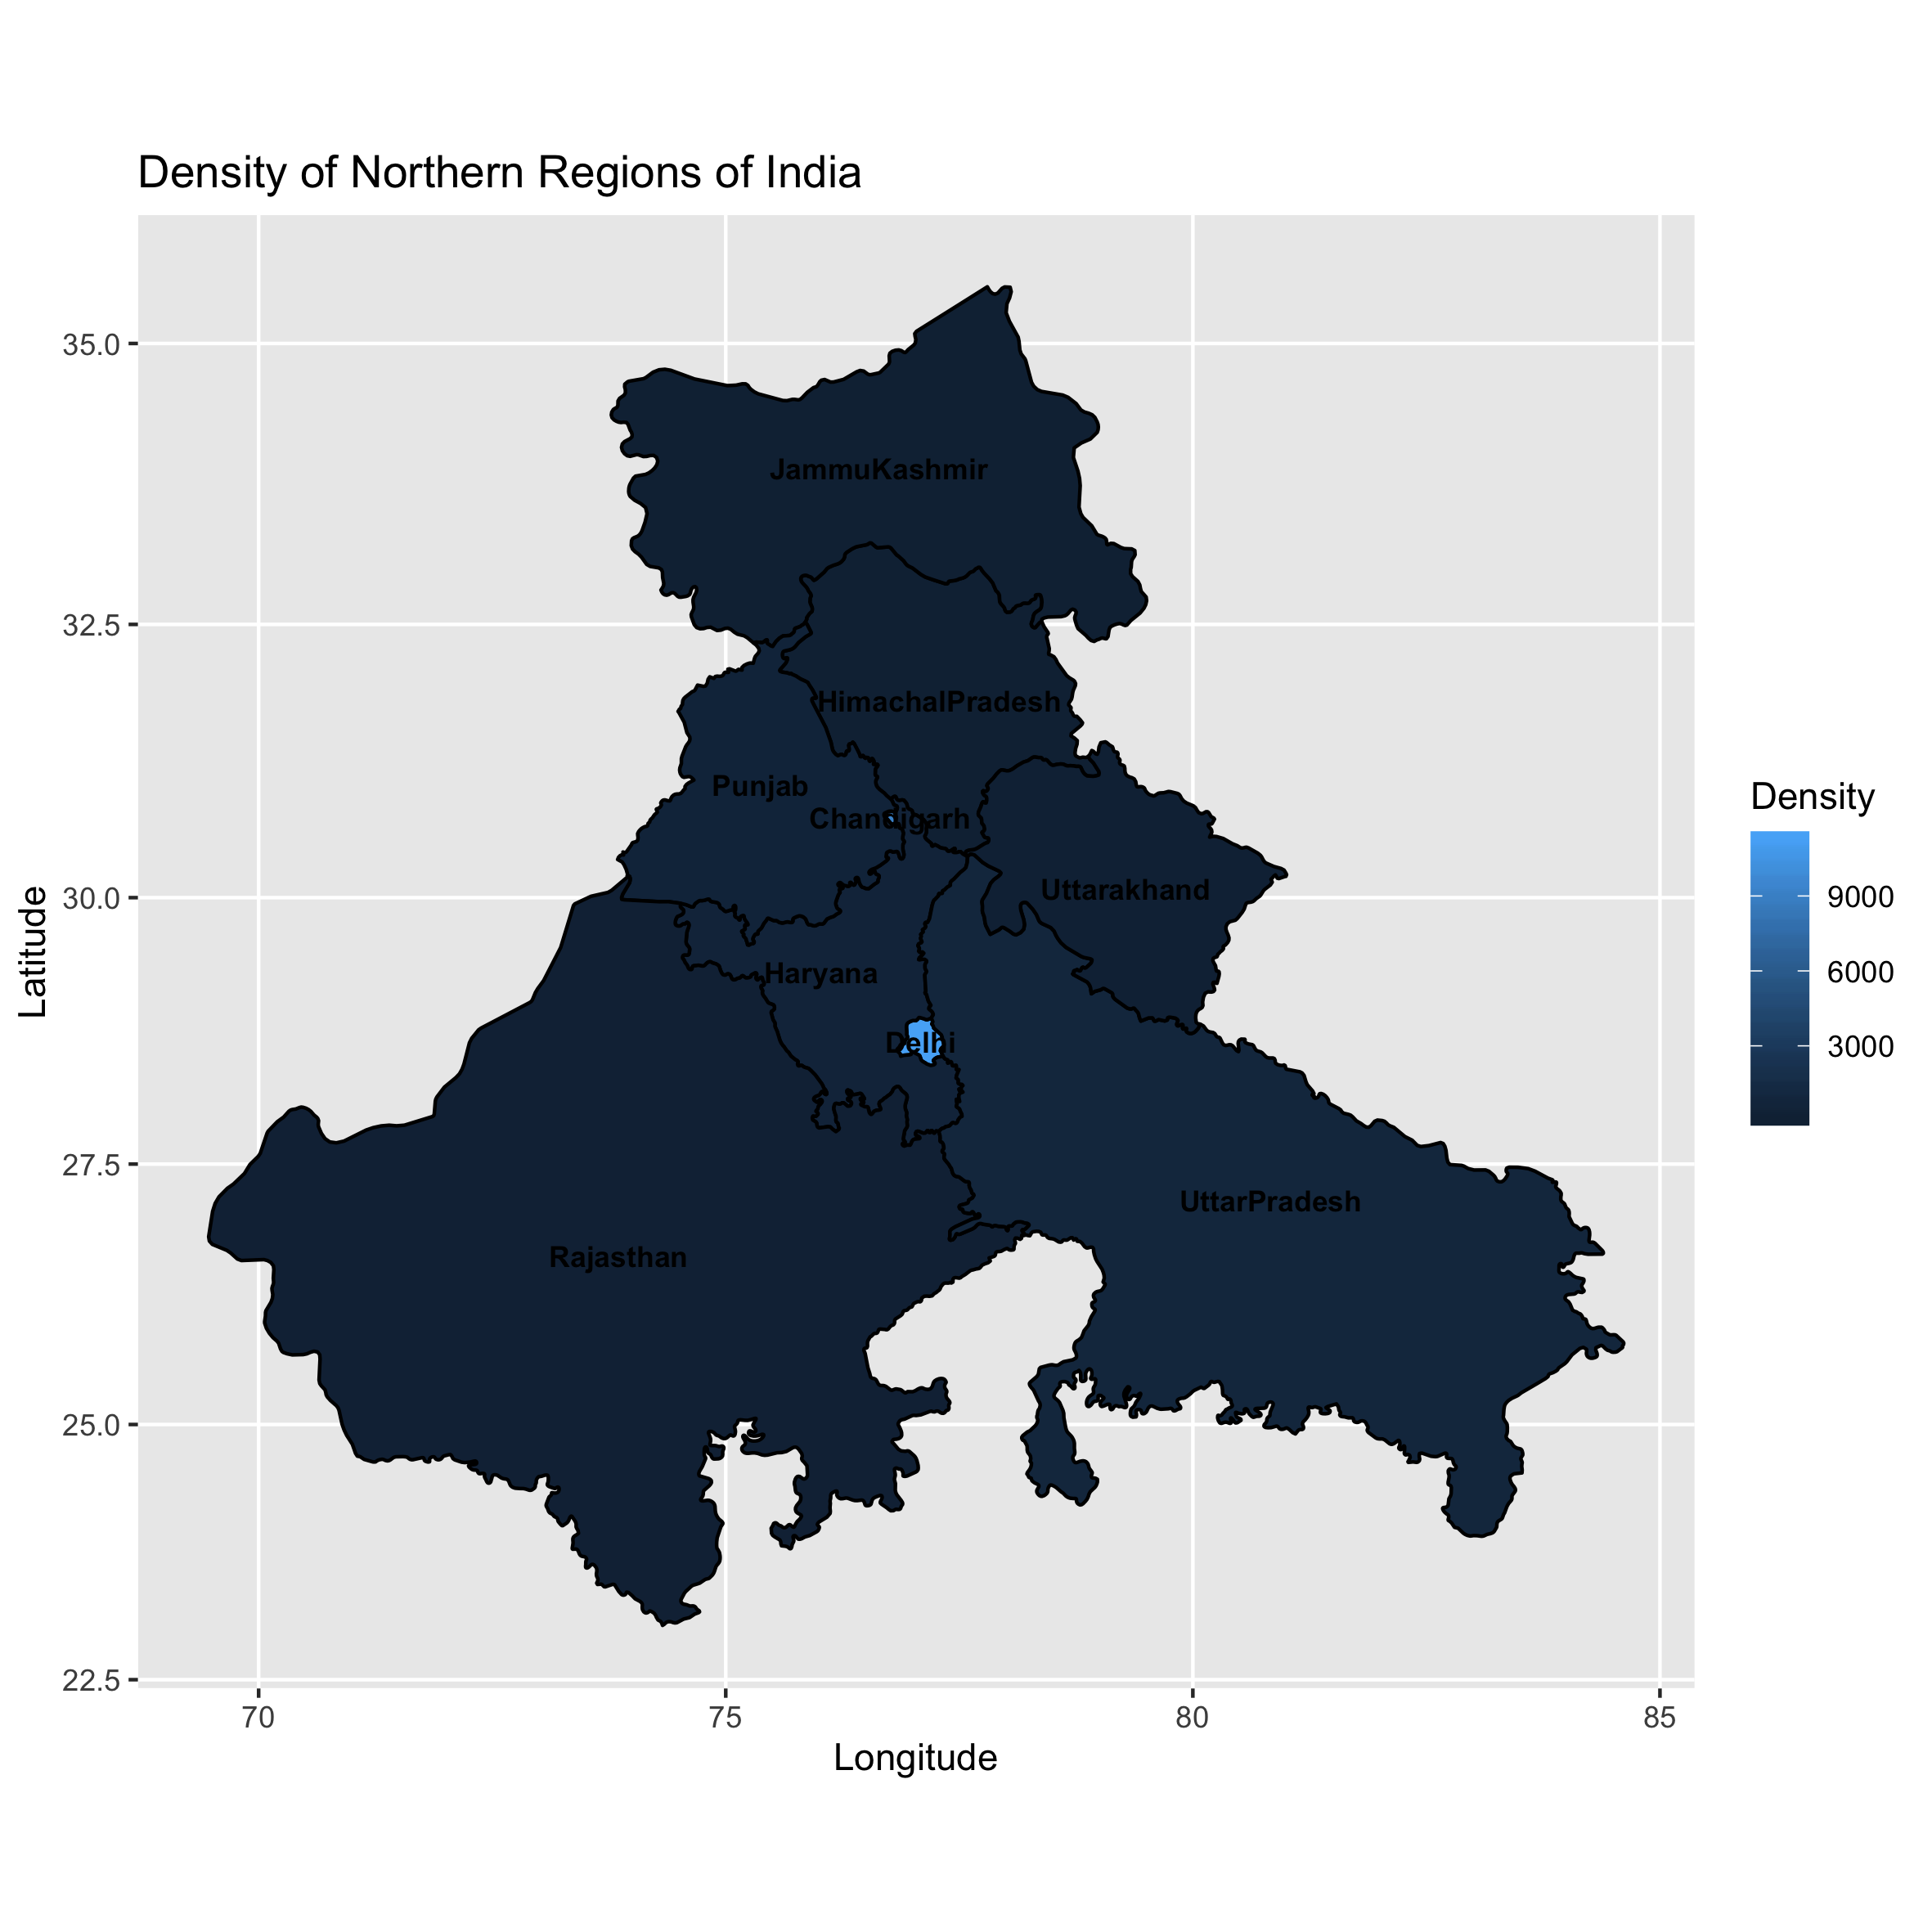
\includegraphics[scale = 0.095]{den.png}
\end{frame}
%---------------------------------------------%
%% SLIDE 1.4.2:
\begin{frame}
	\frametitle{Exploratory Data Analysis: Demographic features (2)}
	\framesubtitle{Large rural, small urban states}
	\center 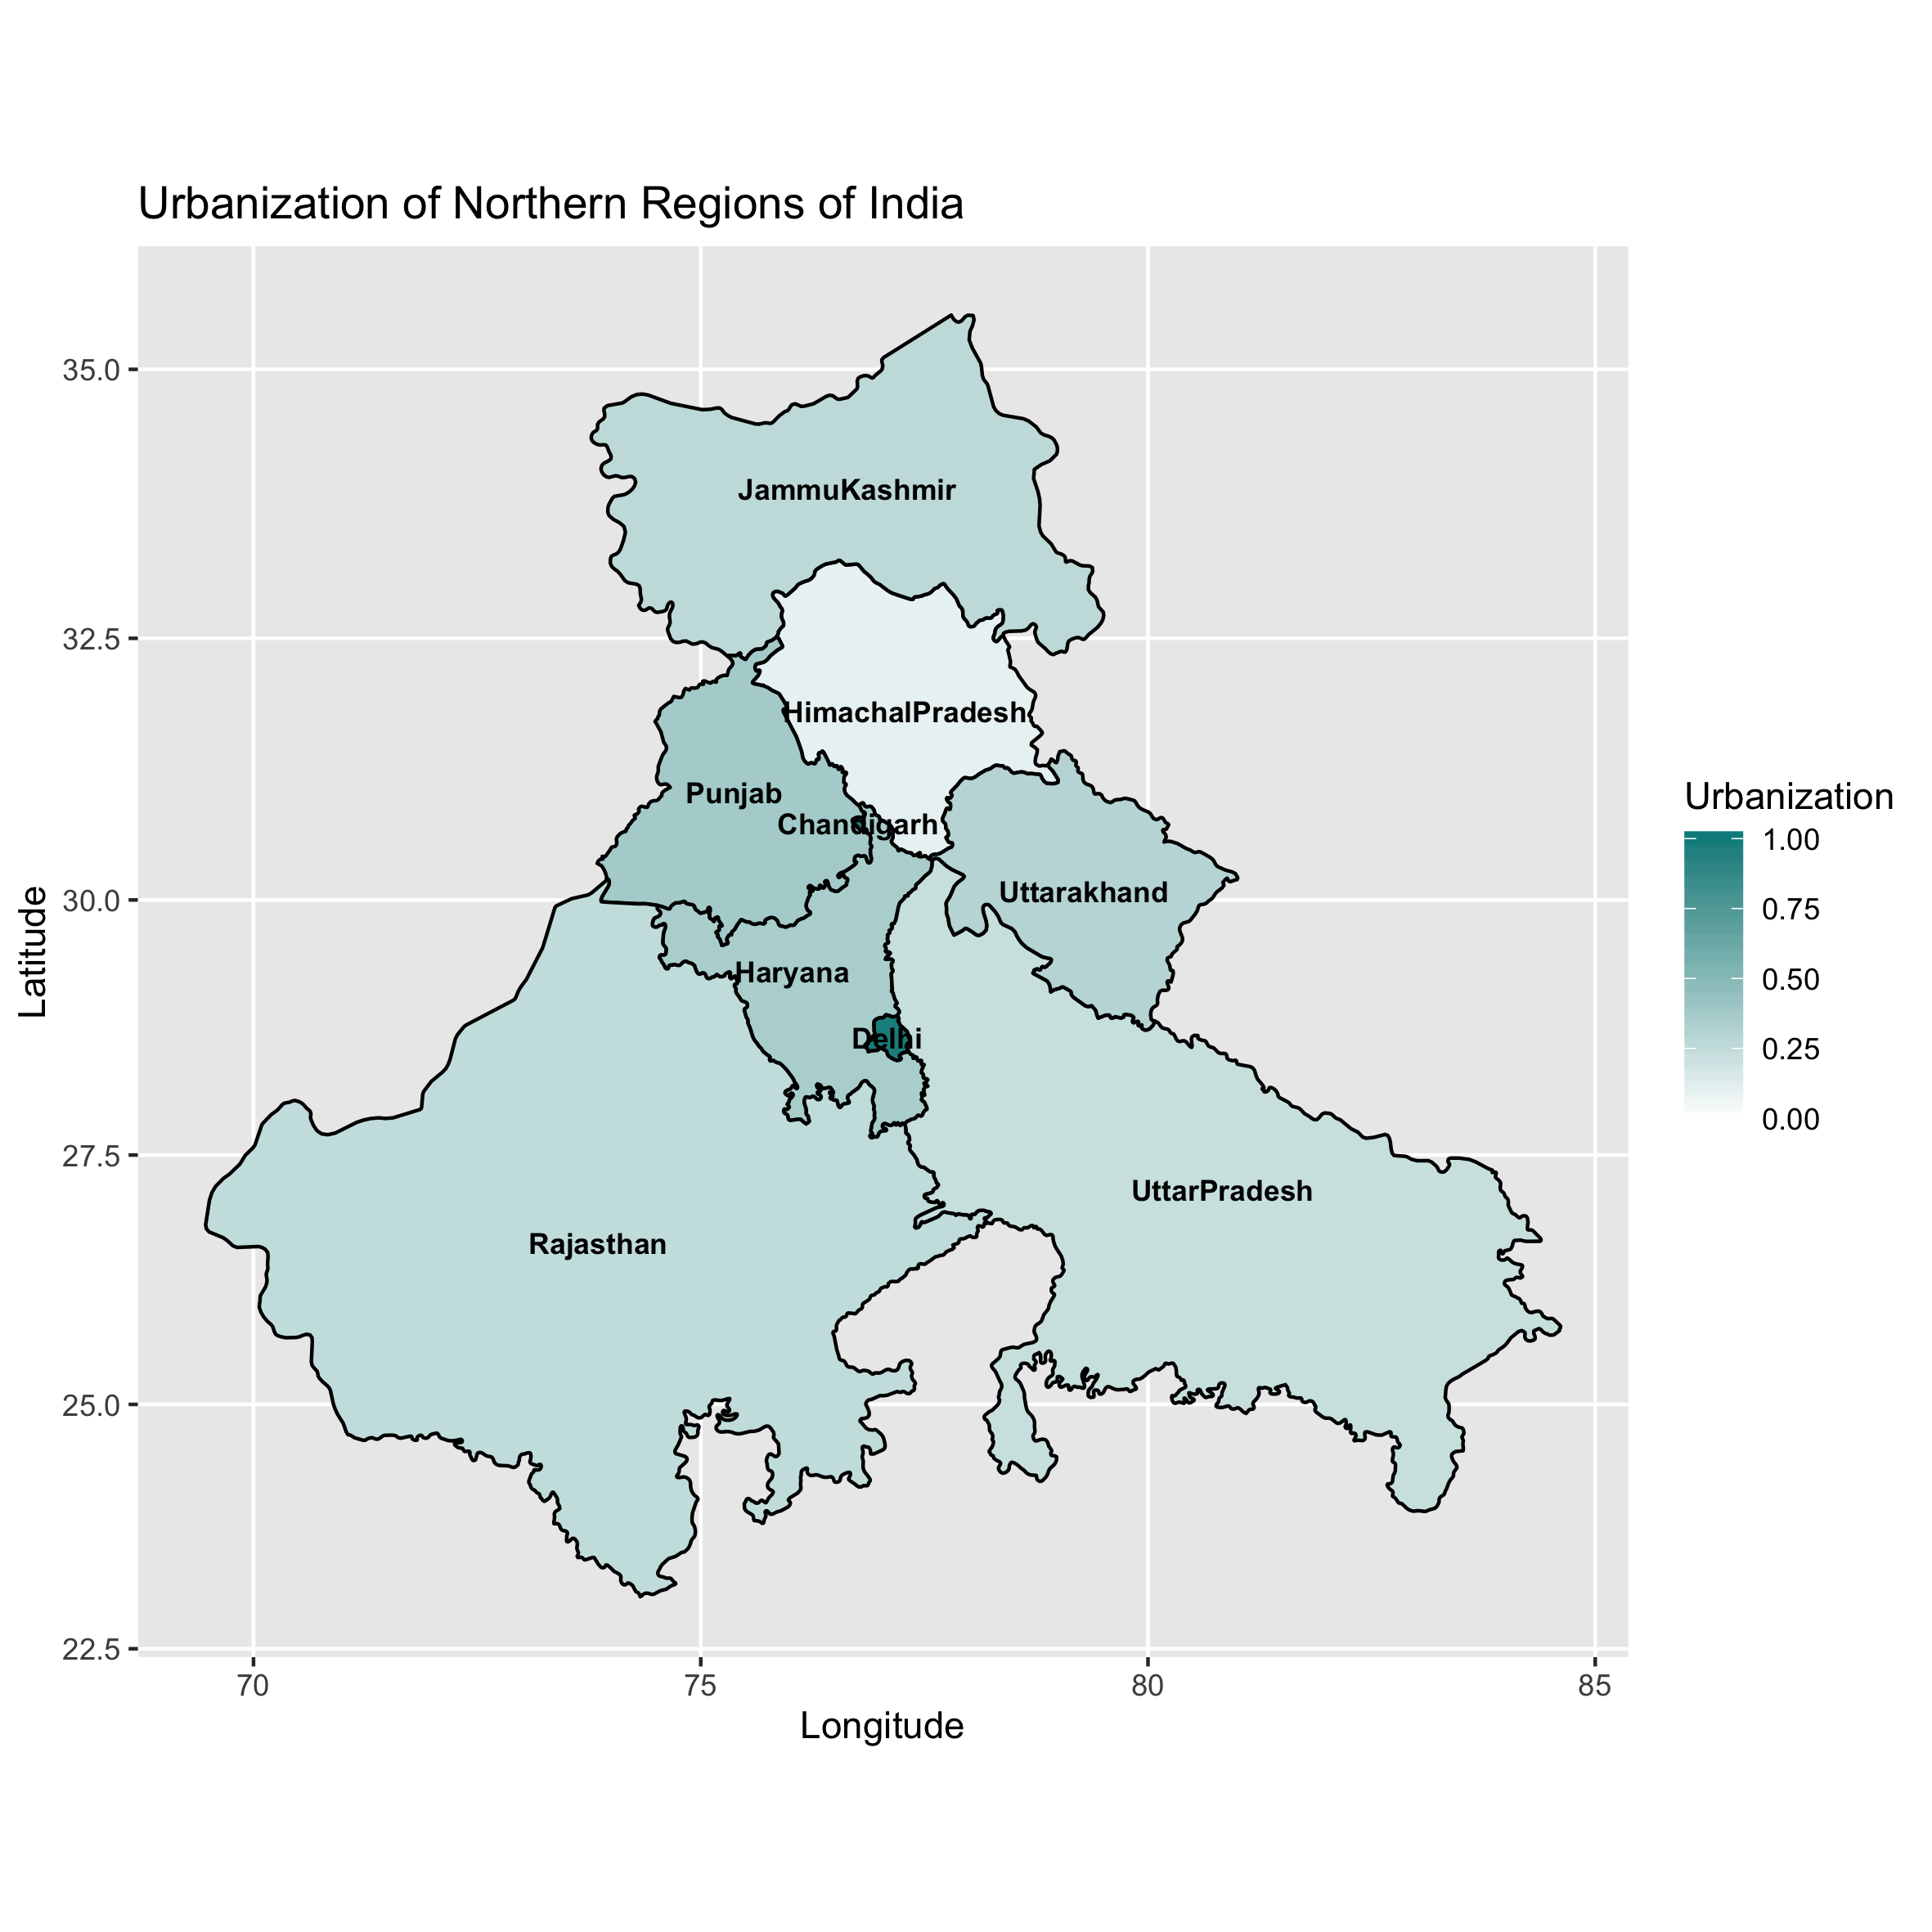
\includegraphics[scale = 0.1]{urb.png}
\end{frame}
%---------------------------------------------%
%% SLIDE 1.4.3:
\begin{frame}
	\frametitle{Exploratory Data Analysis: Health system organization (1)}
	\framesubtitle{The city is still the center of healthcare}
	\center 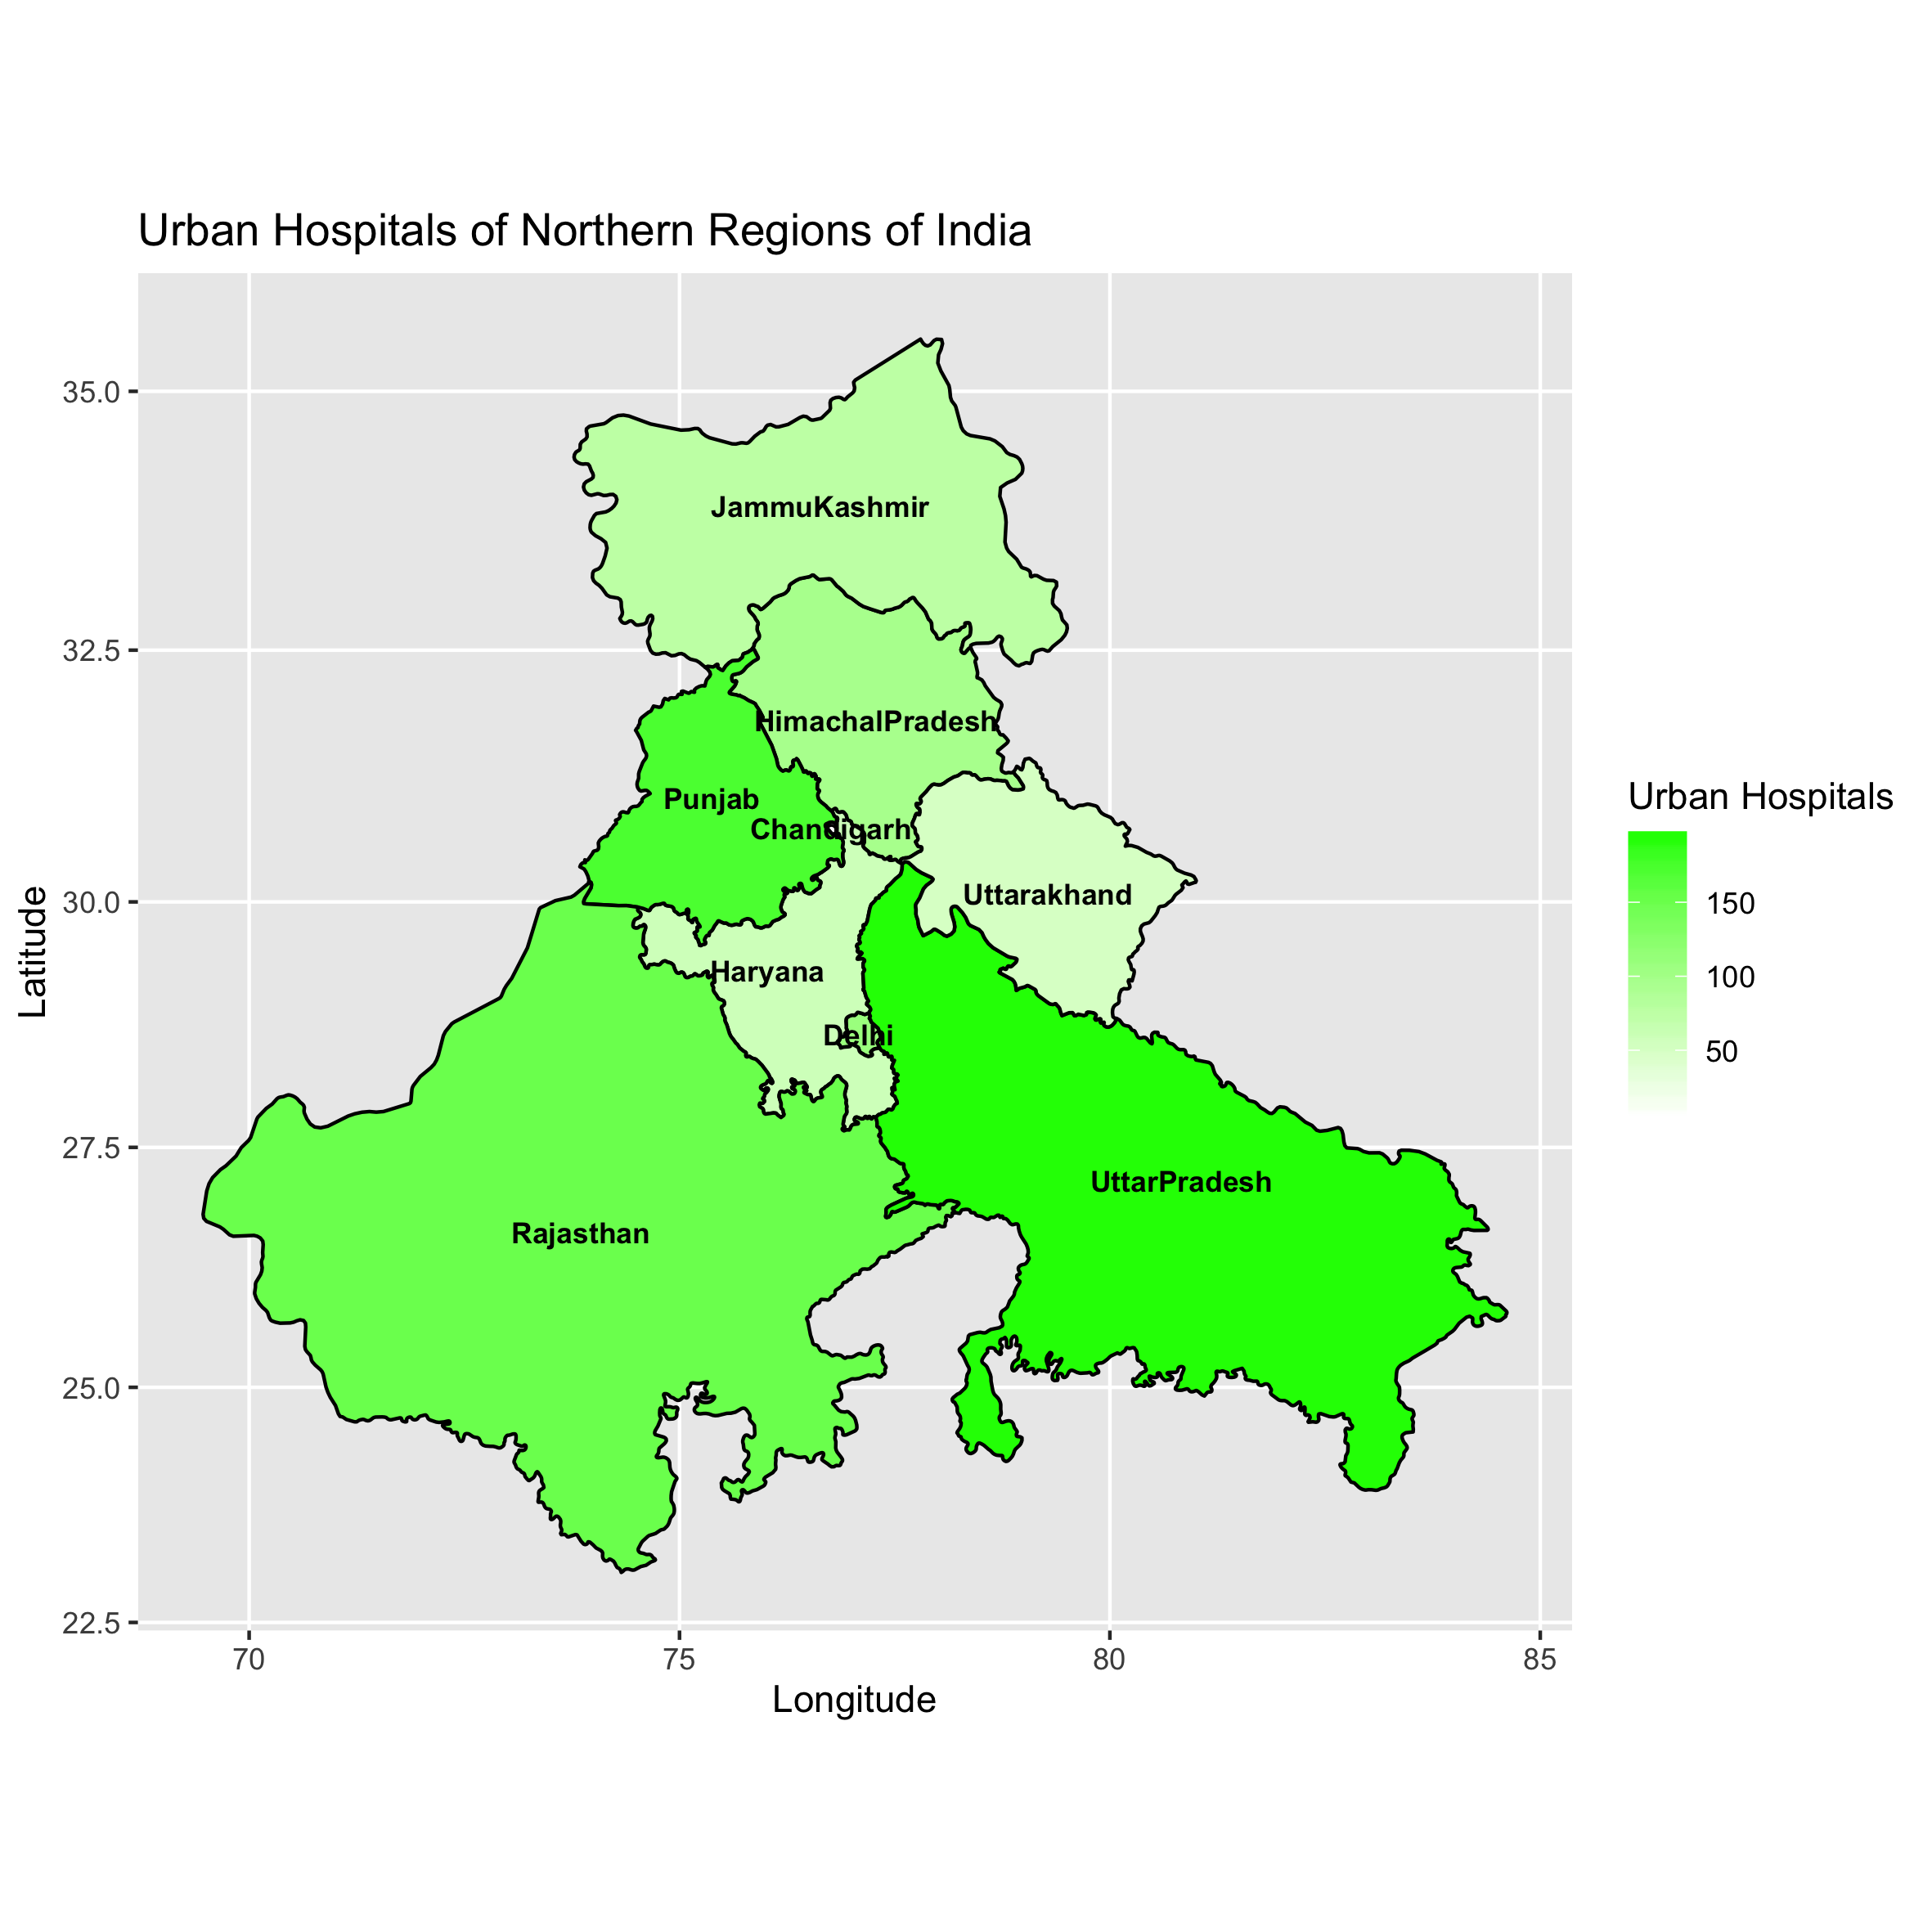
\includegraphics[scale = 0.1]{urbanh.png}
\end{frame}
%---------------------------------------------%
%% SLIDE 1.4.4:
\begin{frame}
	\frametitle{Exploratory Data Analysis: Health system organization (2)}
	\framesubtitle{The city is still the center for healthcare}
	\center 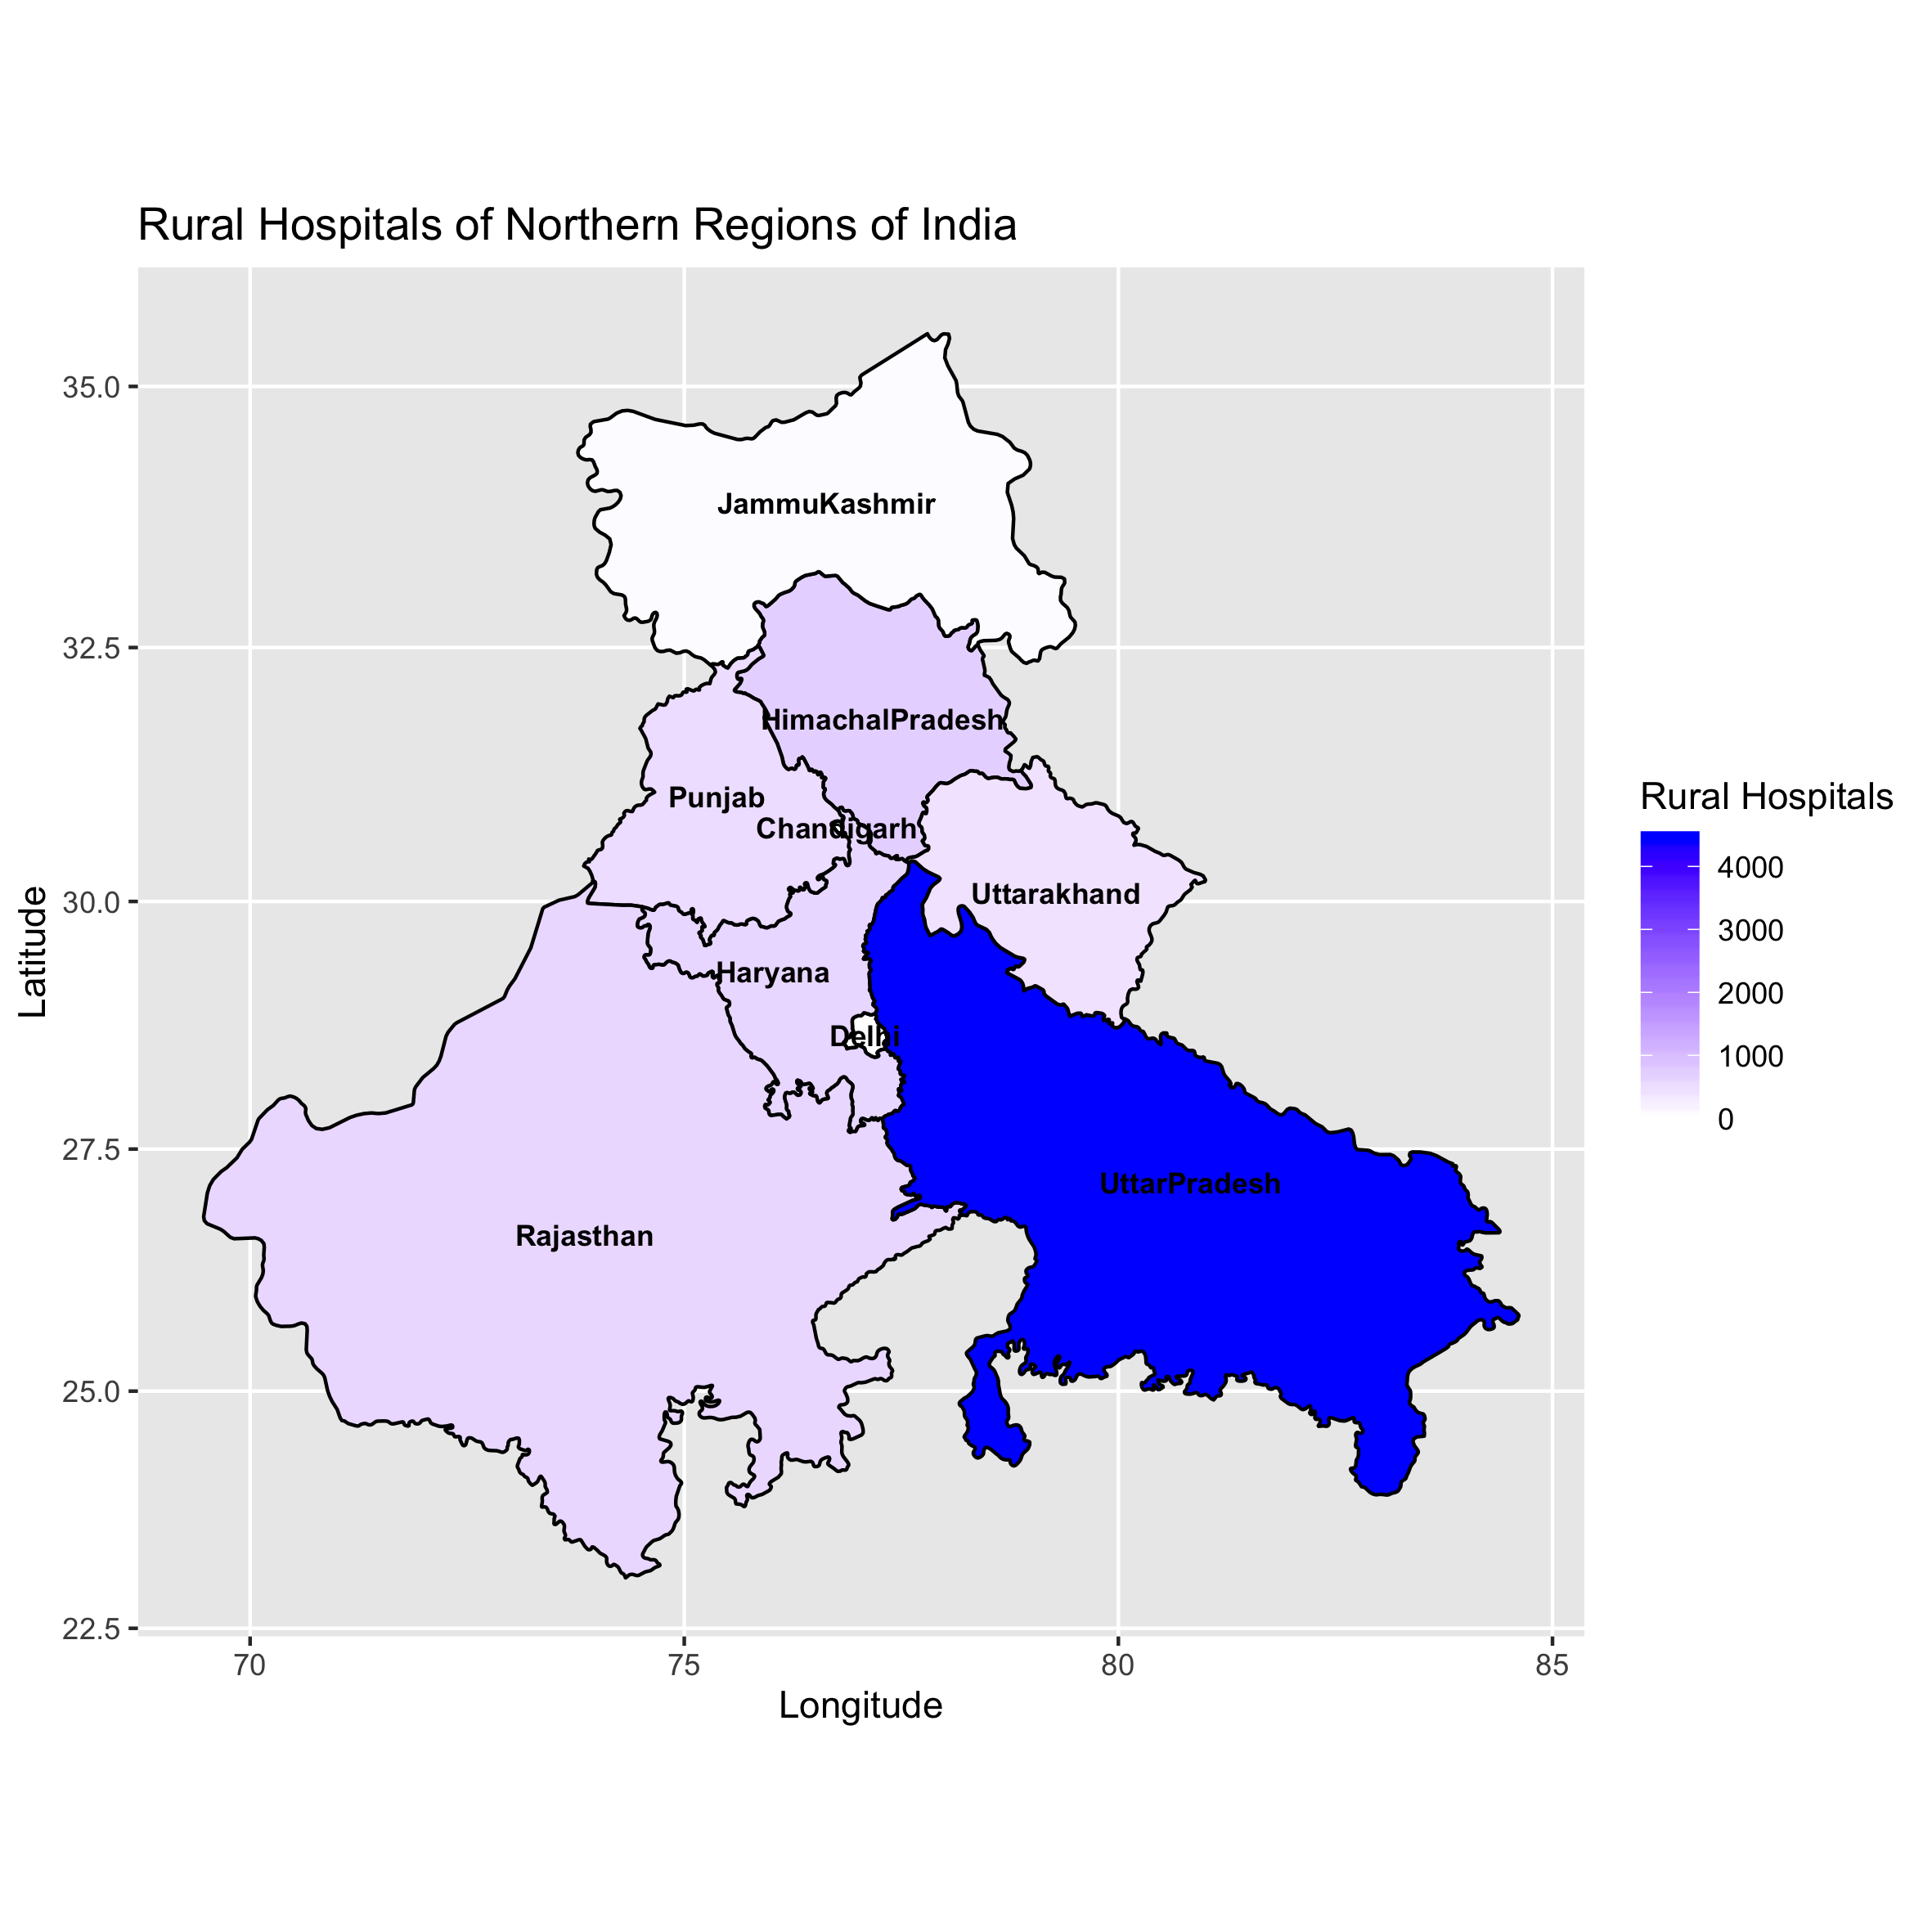
\includegraphics[scale = 0.1]{ruralh.png}
\end{frame}
%---------------------------------------------%
%% SLIDE 1.4.5:
\begin{frame}
	\frametitle{Exploratory Data Analysis: $\#$ positive cases per region}
	\framesubtitle{Not always a matter of population / landsize}
	\center 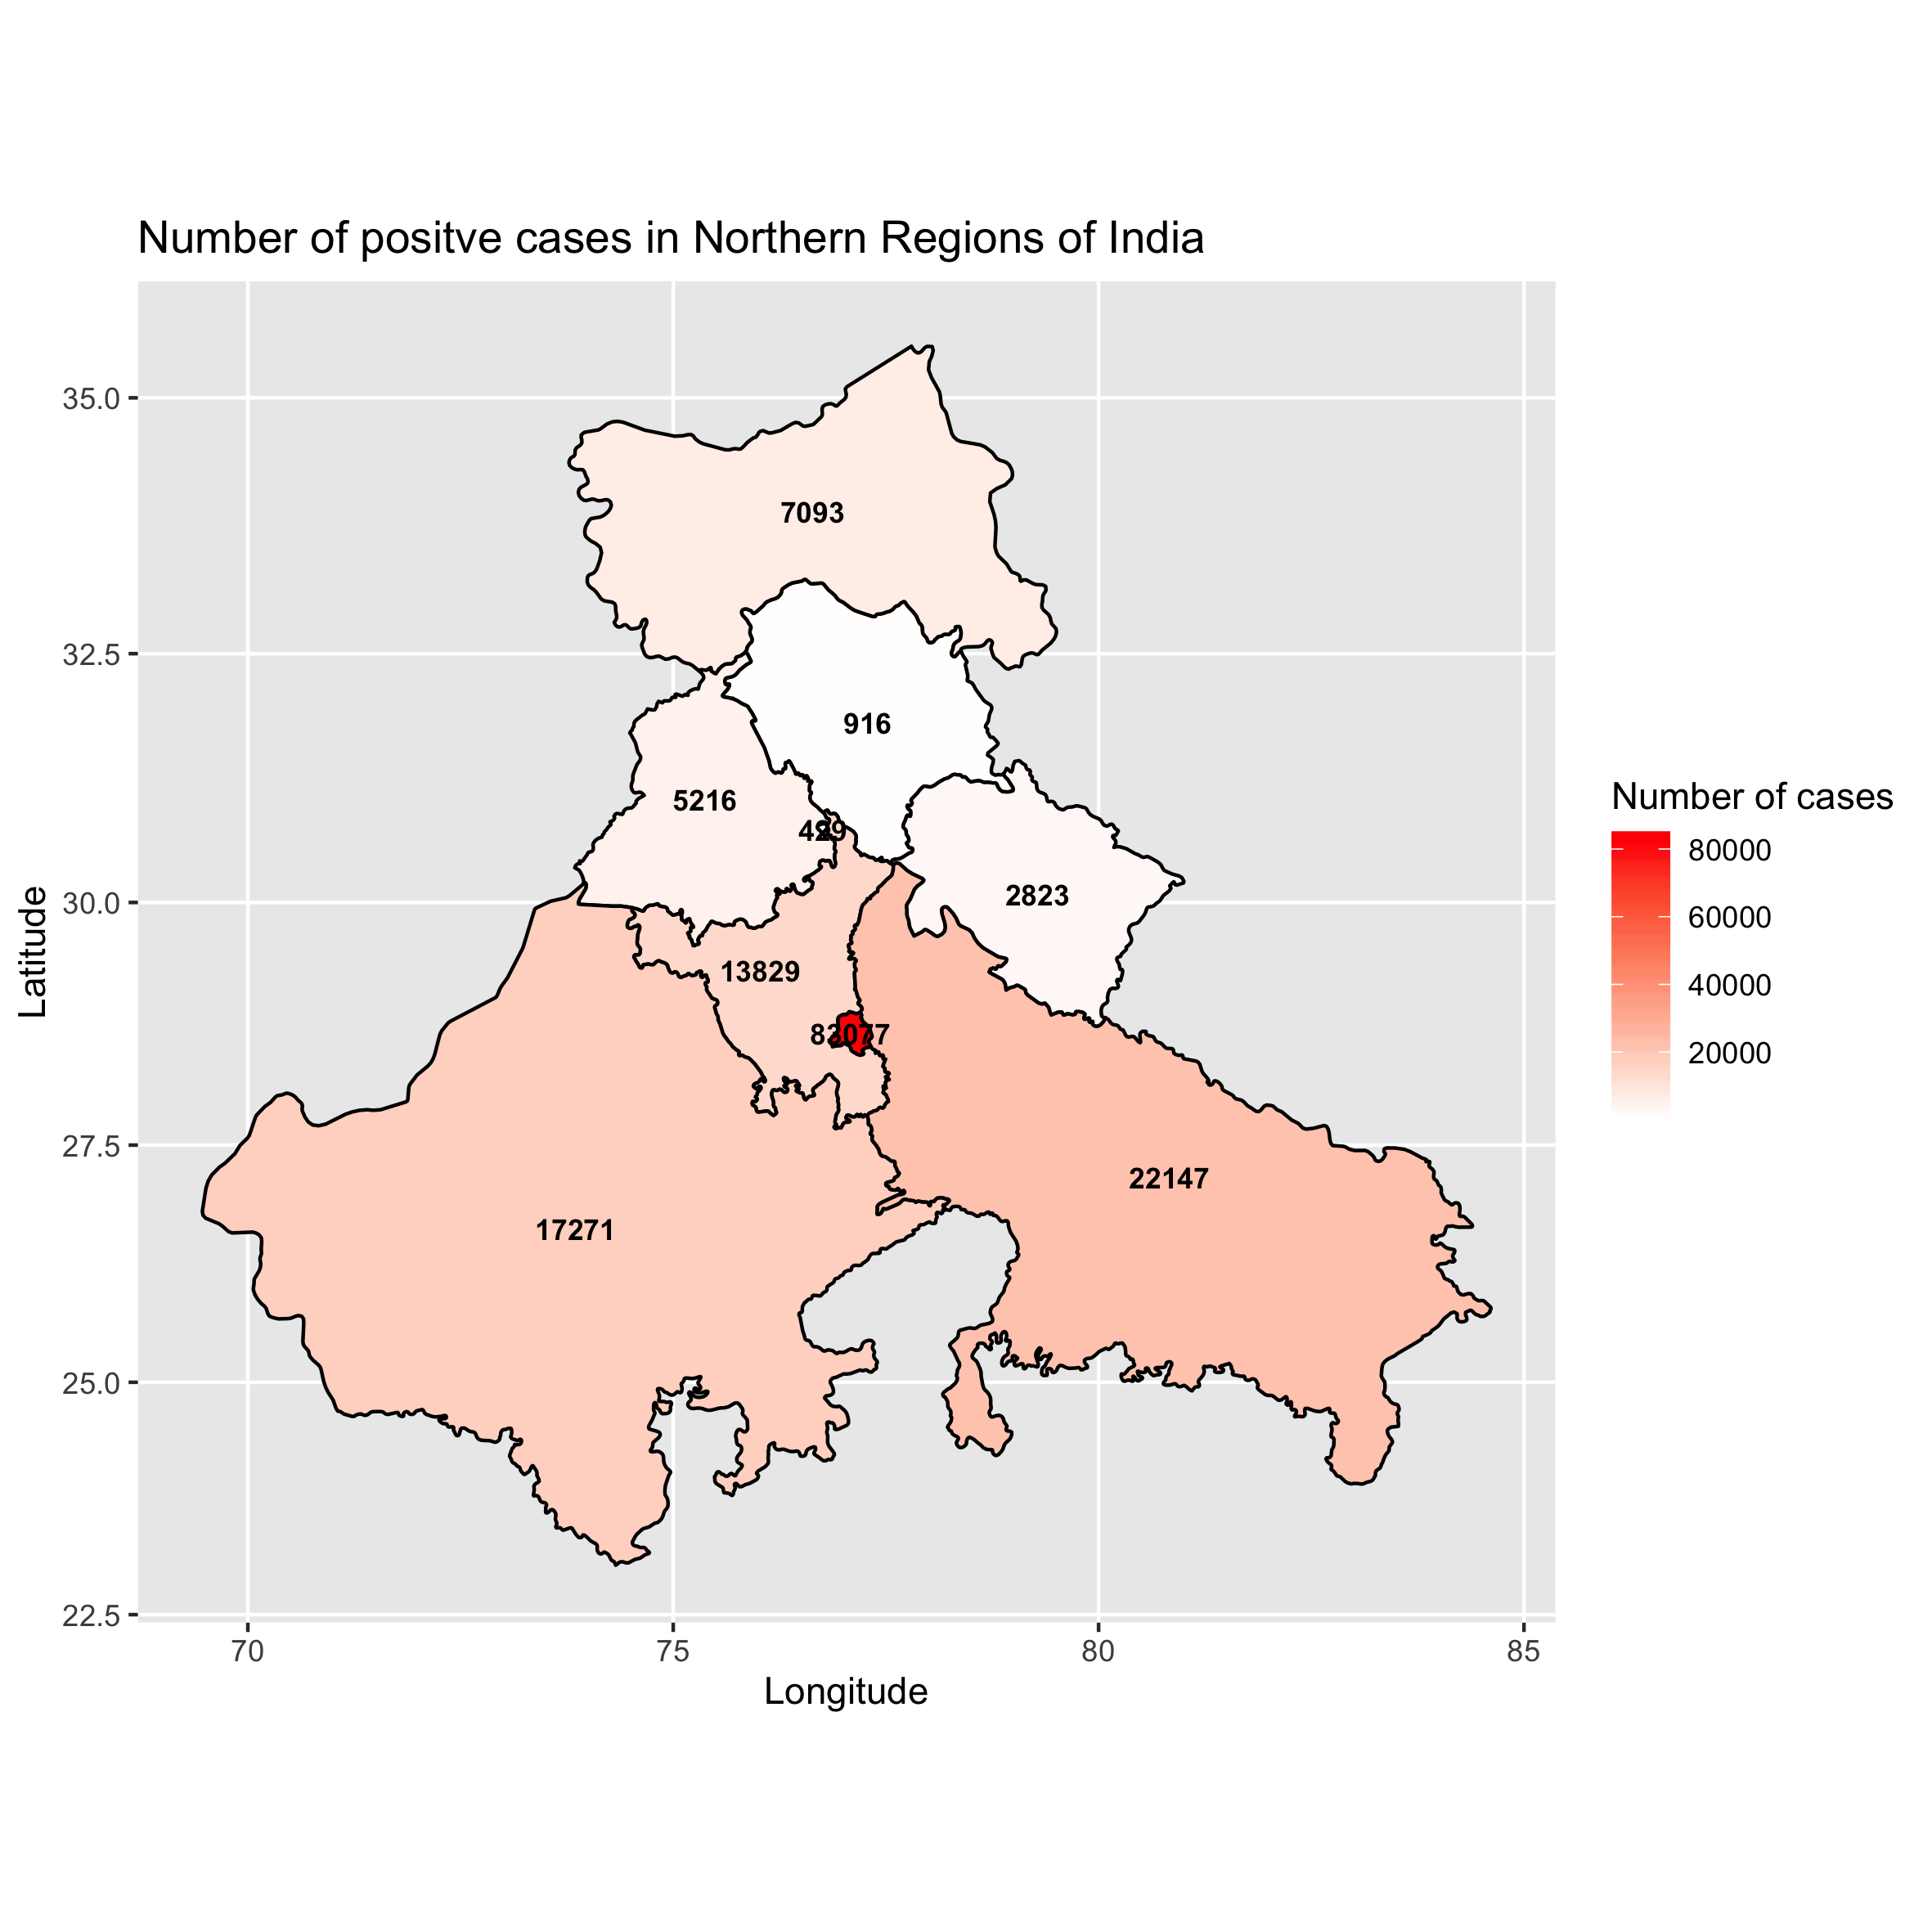
\includegraphics[scale = 0.1]{pos.png}
\end{frame}
%---------------------------------------------%
%% SLIDE 1.4.6:
\begin{frame}
	\frametitle{Exploratory Data Analysis: Trend of positive cases}
	\framesubtitle{An exponential trend, maybe?}
	\center 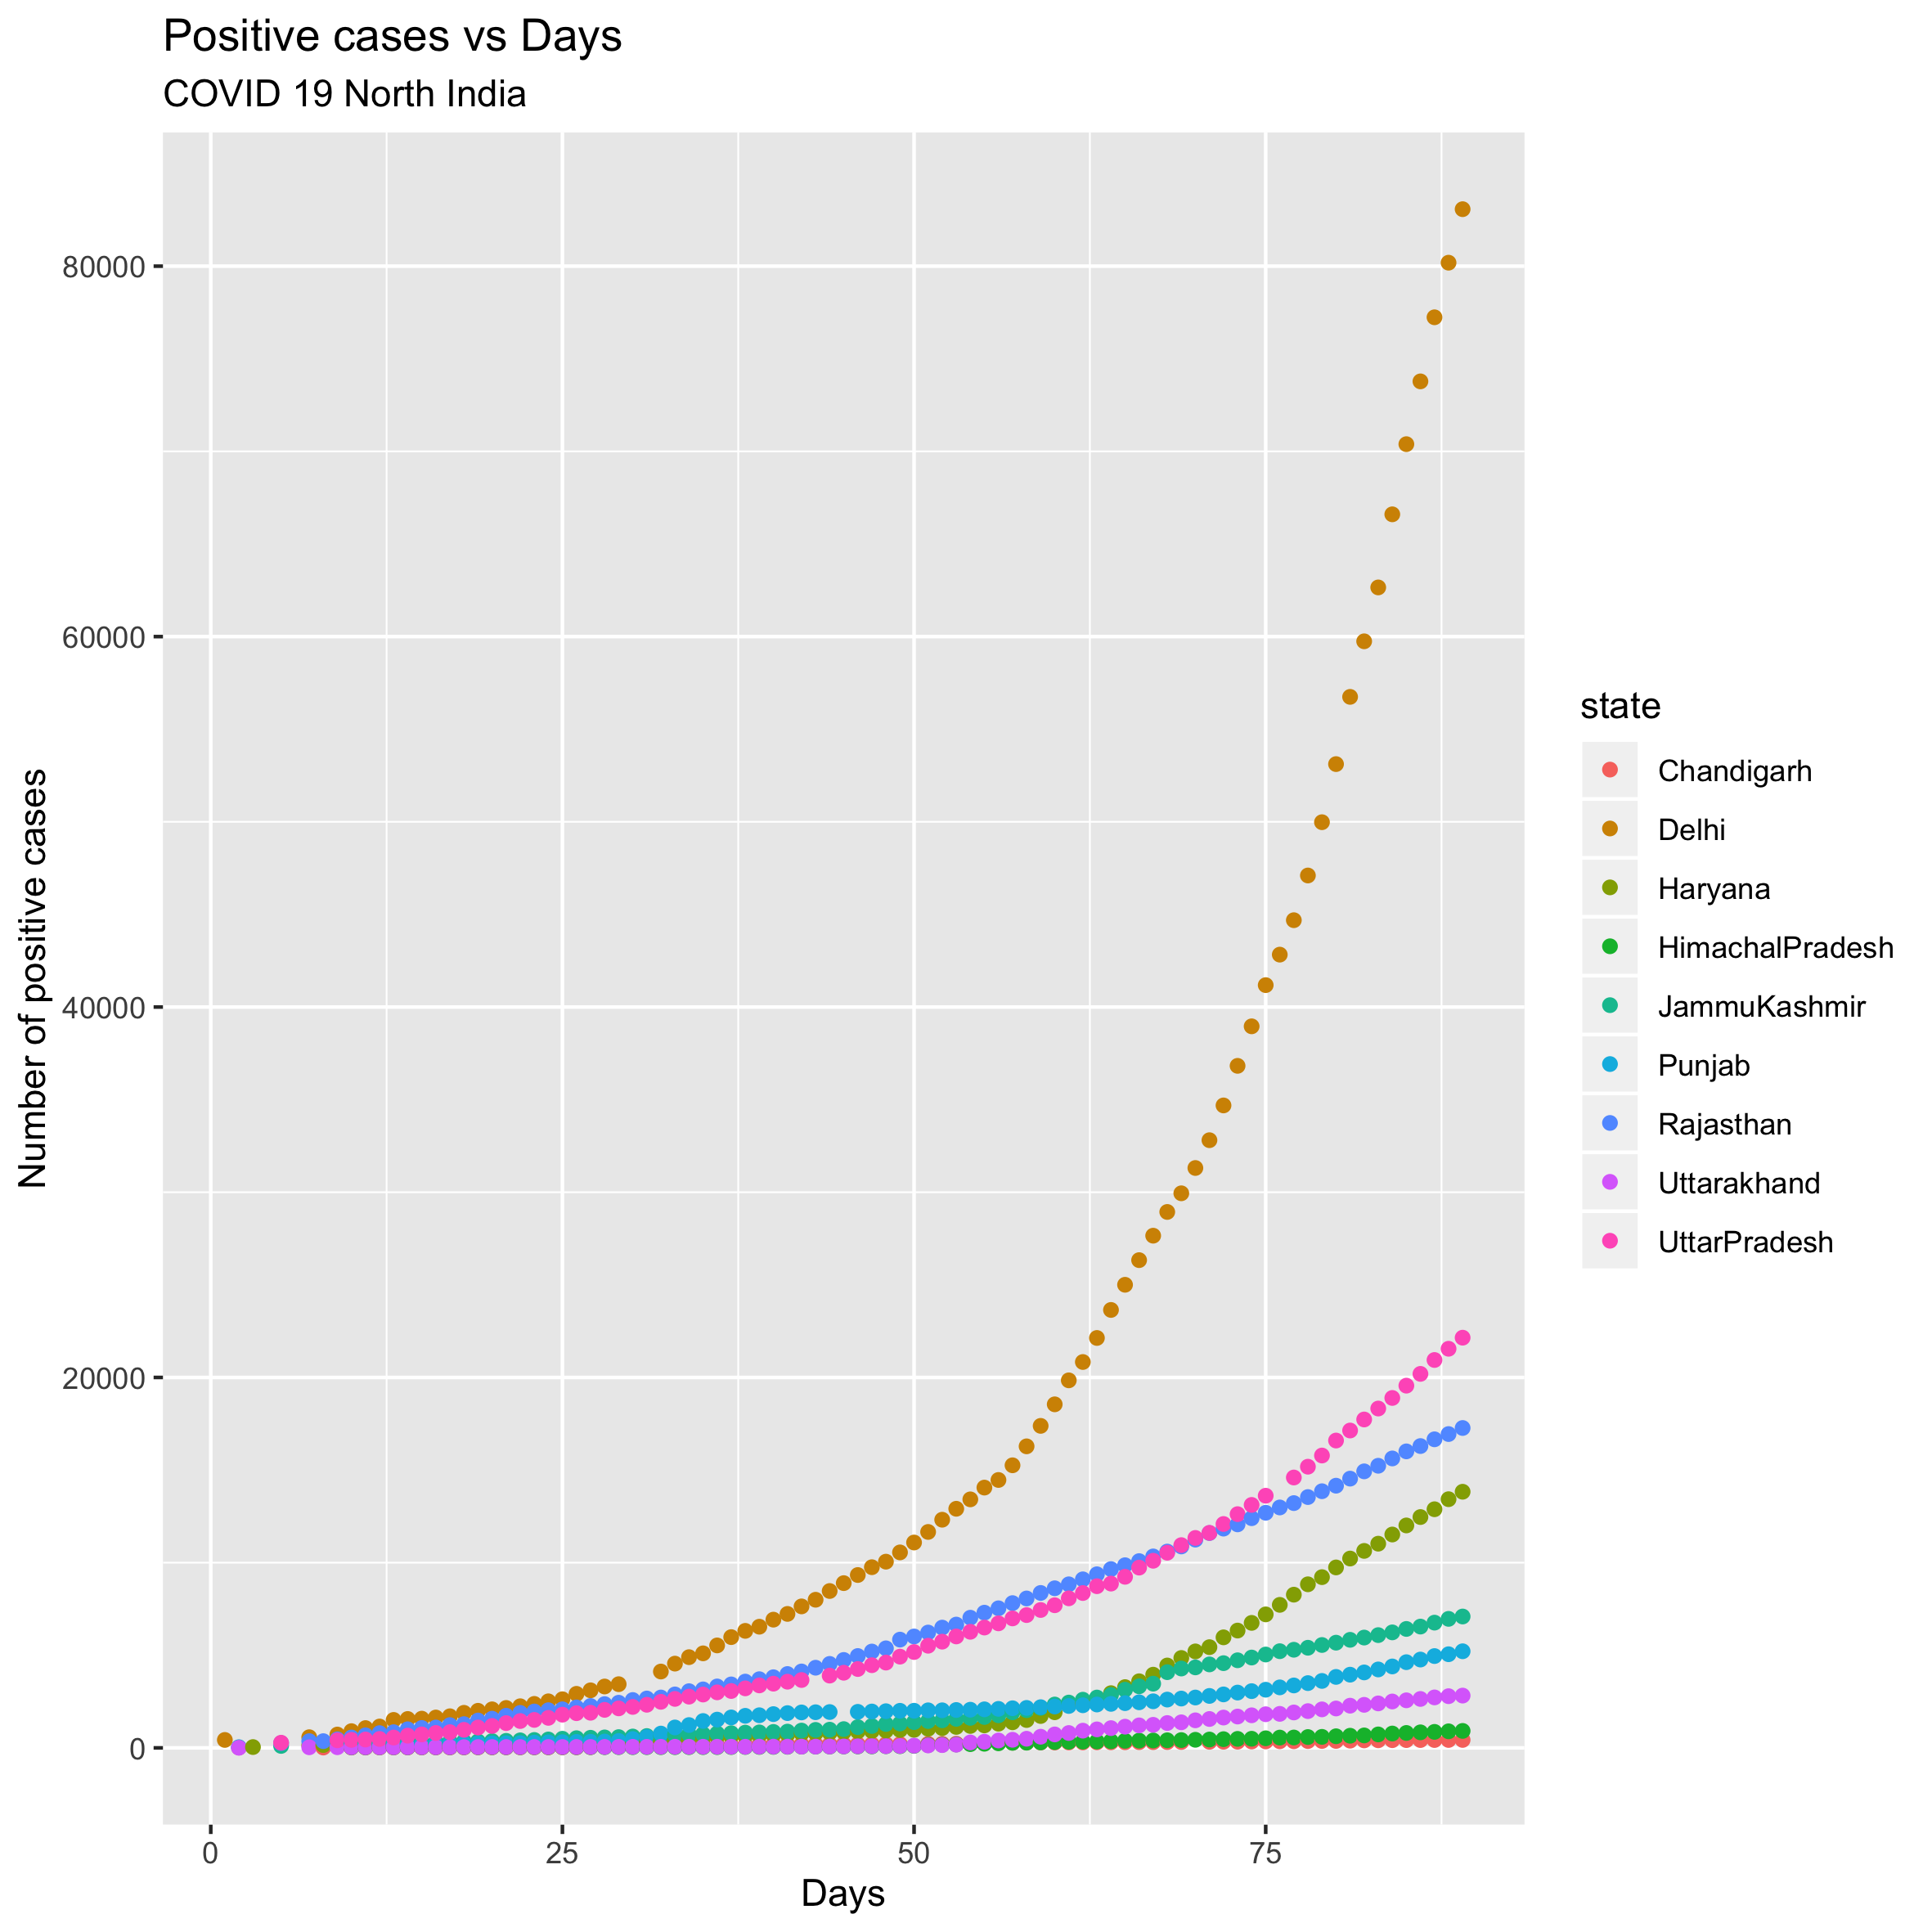
\includegraphics[scale = 0.085]{pos_date.png}
\end{frame}
%---------------------------------------------%
%% SLIDE 1.4.7:
\begin{frame}
	\frametitle{Exploratory Data Analysis: Trend of average age}
	\framesubtitle{The more vulnerable suffer the most}
	\center 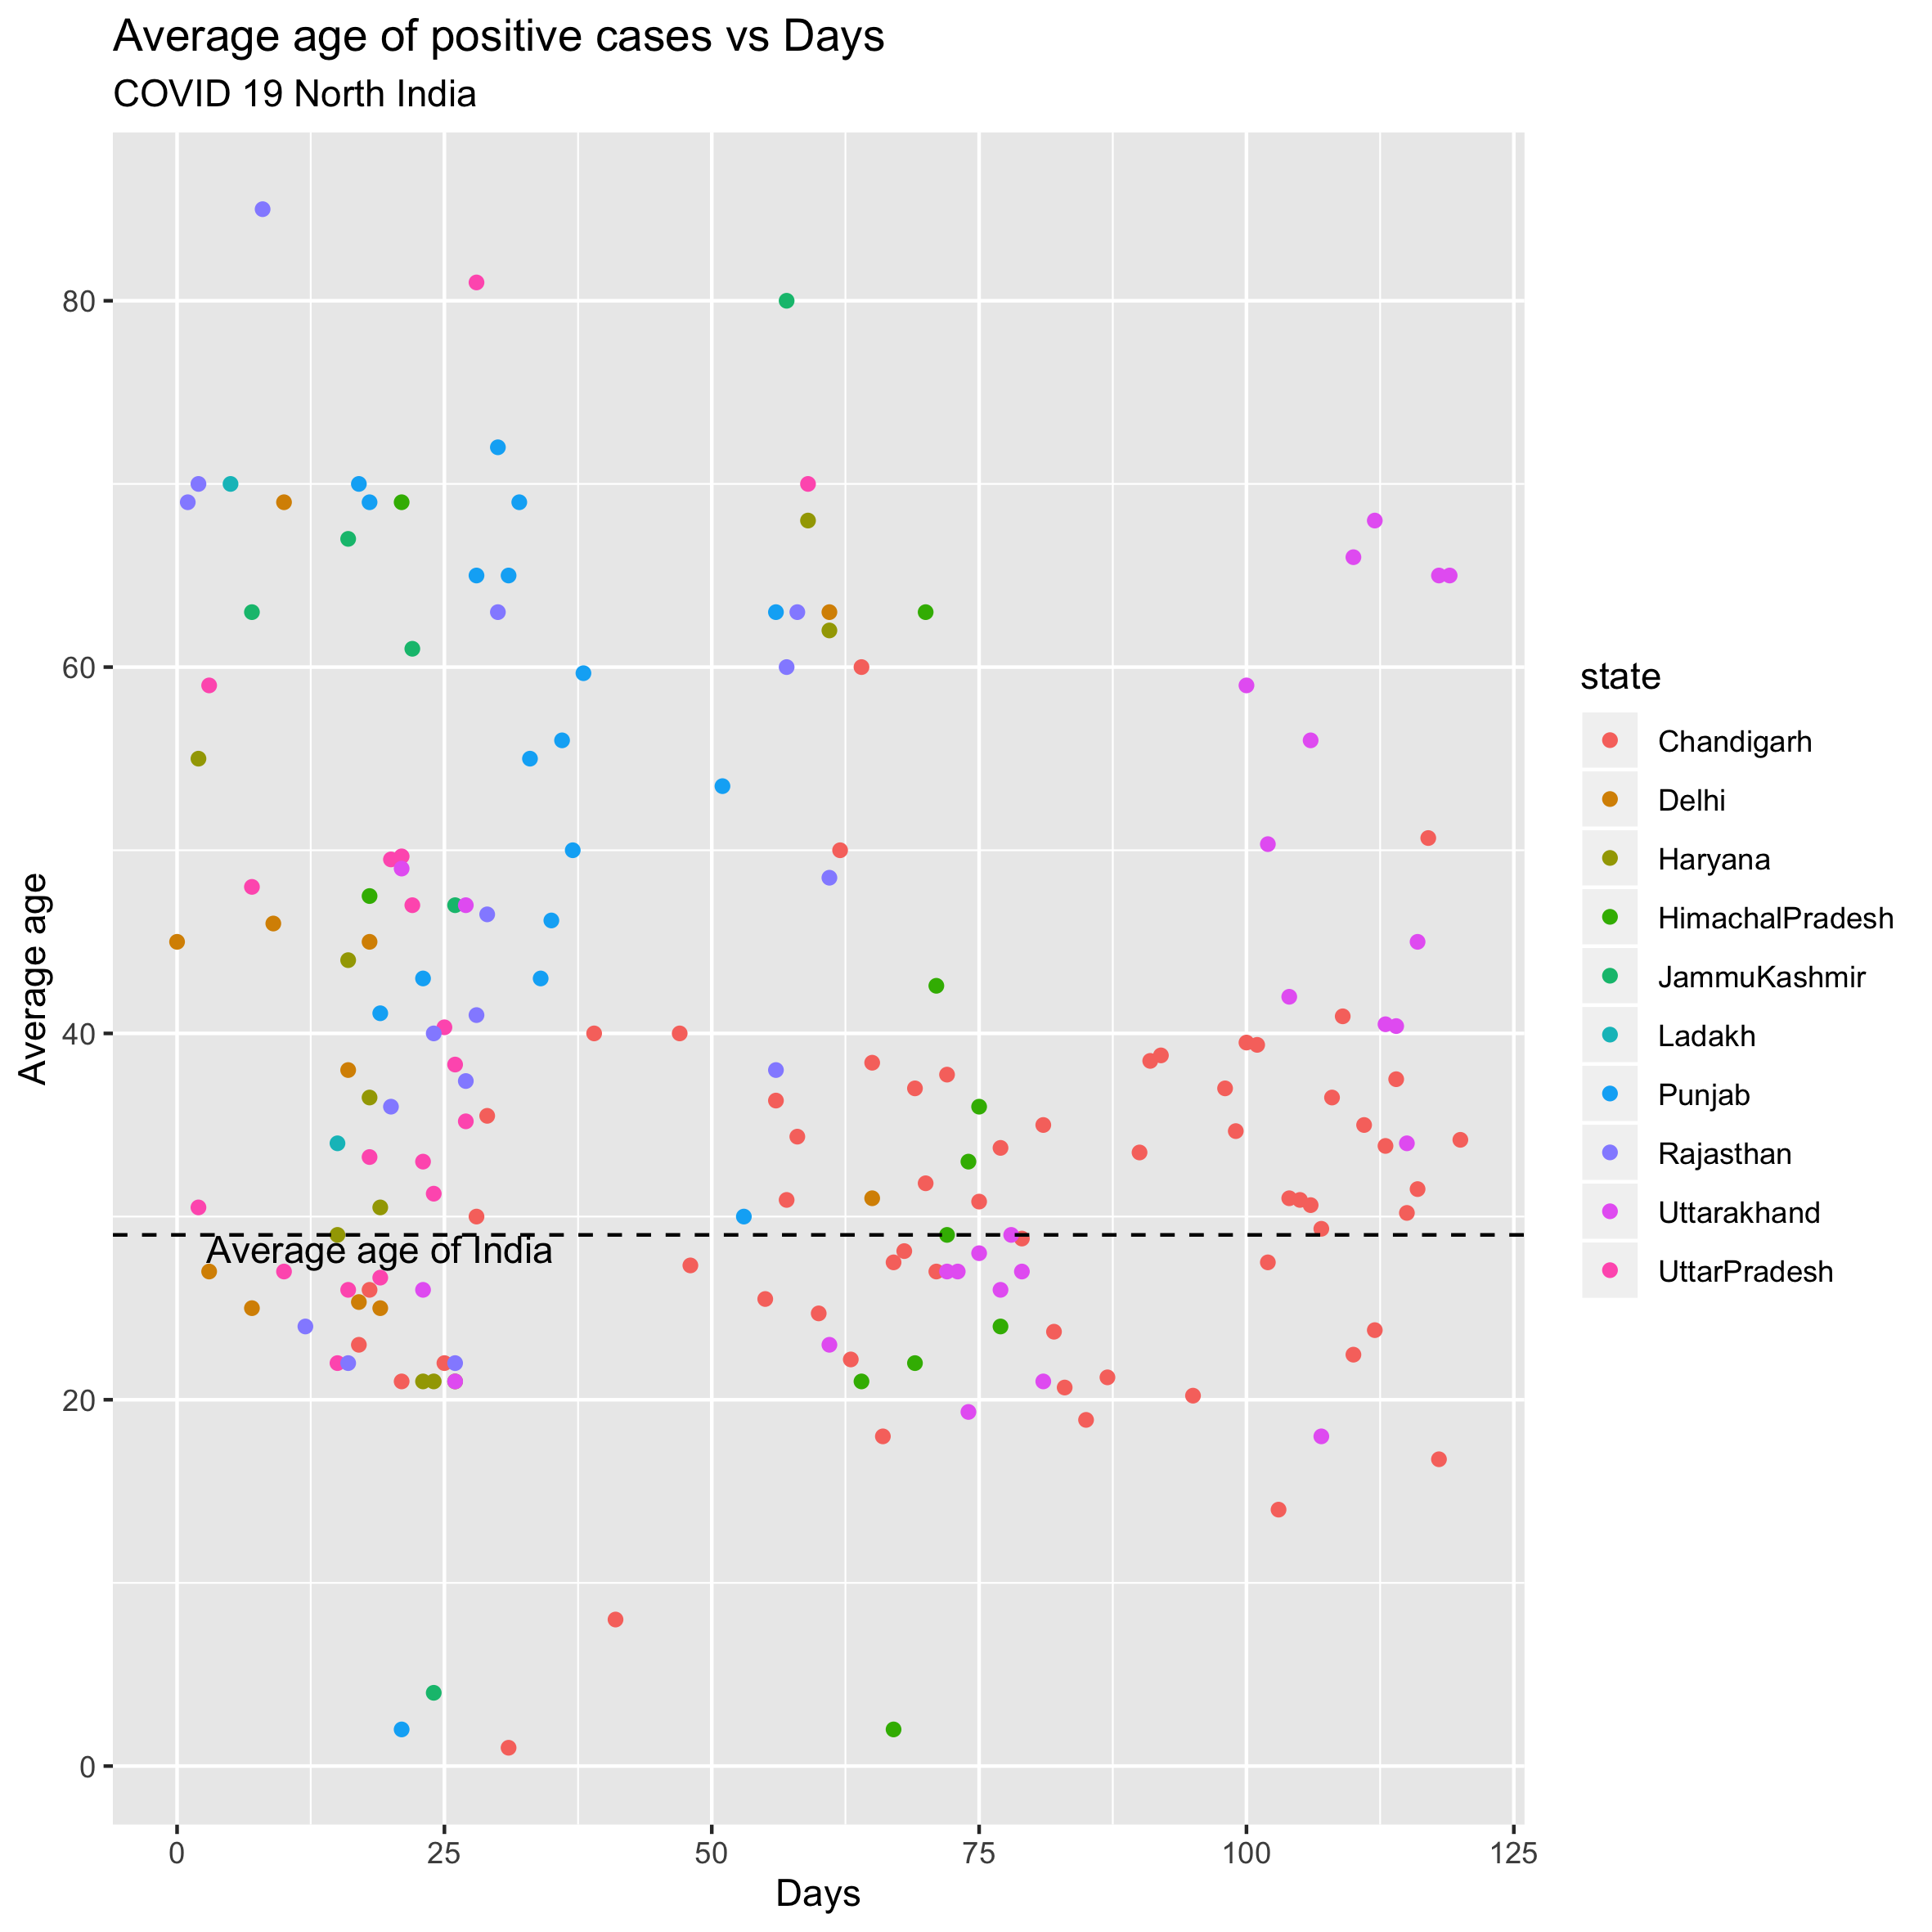
\includegraphics[scale = 0.085]{avg_age_pos.png}
\end{frame}
%---------------------------------------------%
%% SLIDE 1.4.8:
\begin{frame}
	\frametitle{Exploratory Data Analysis: Trend of average sex}
	\framesubtitle{No evident sex prevalence}
	\center 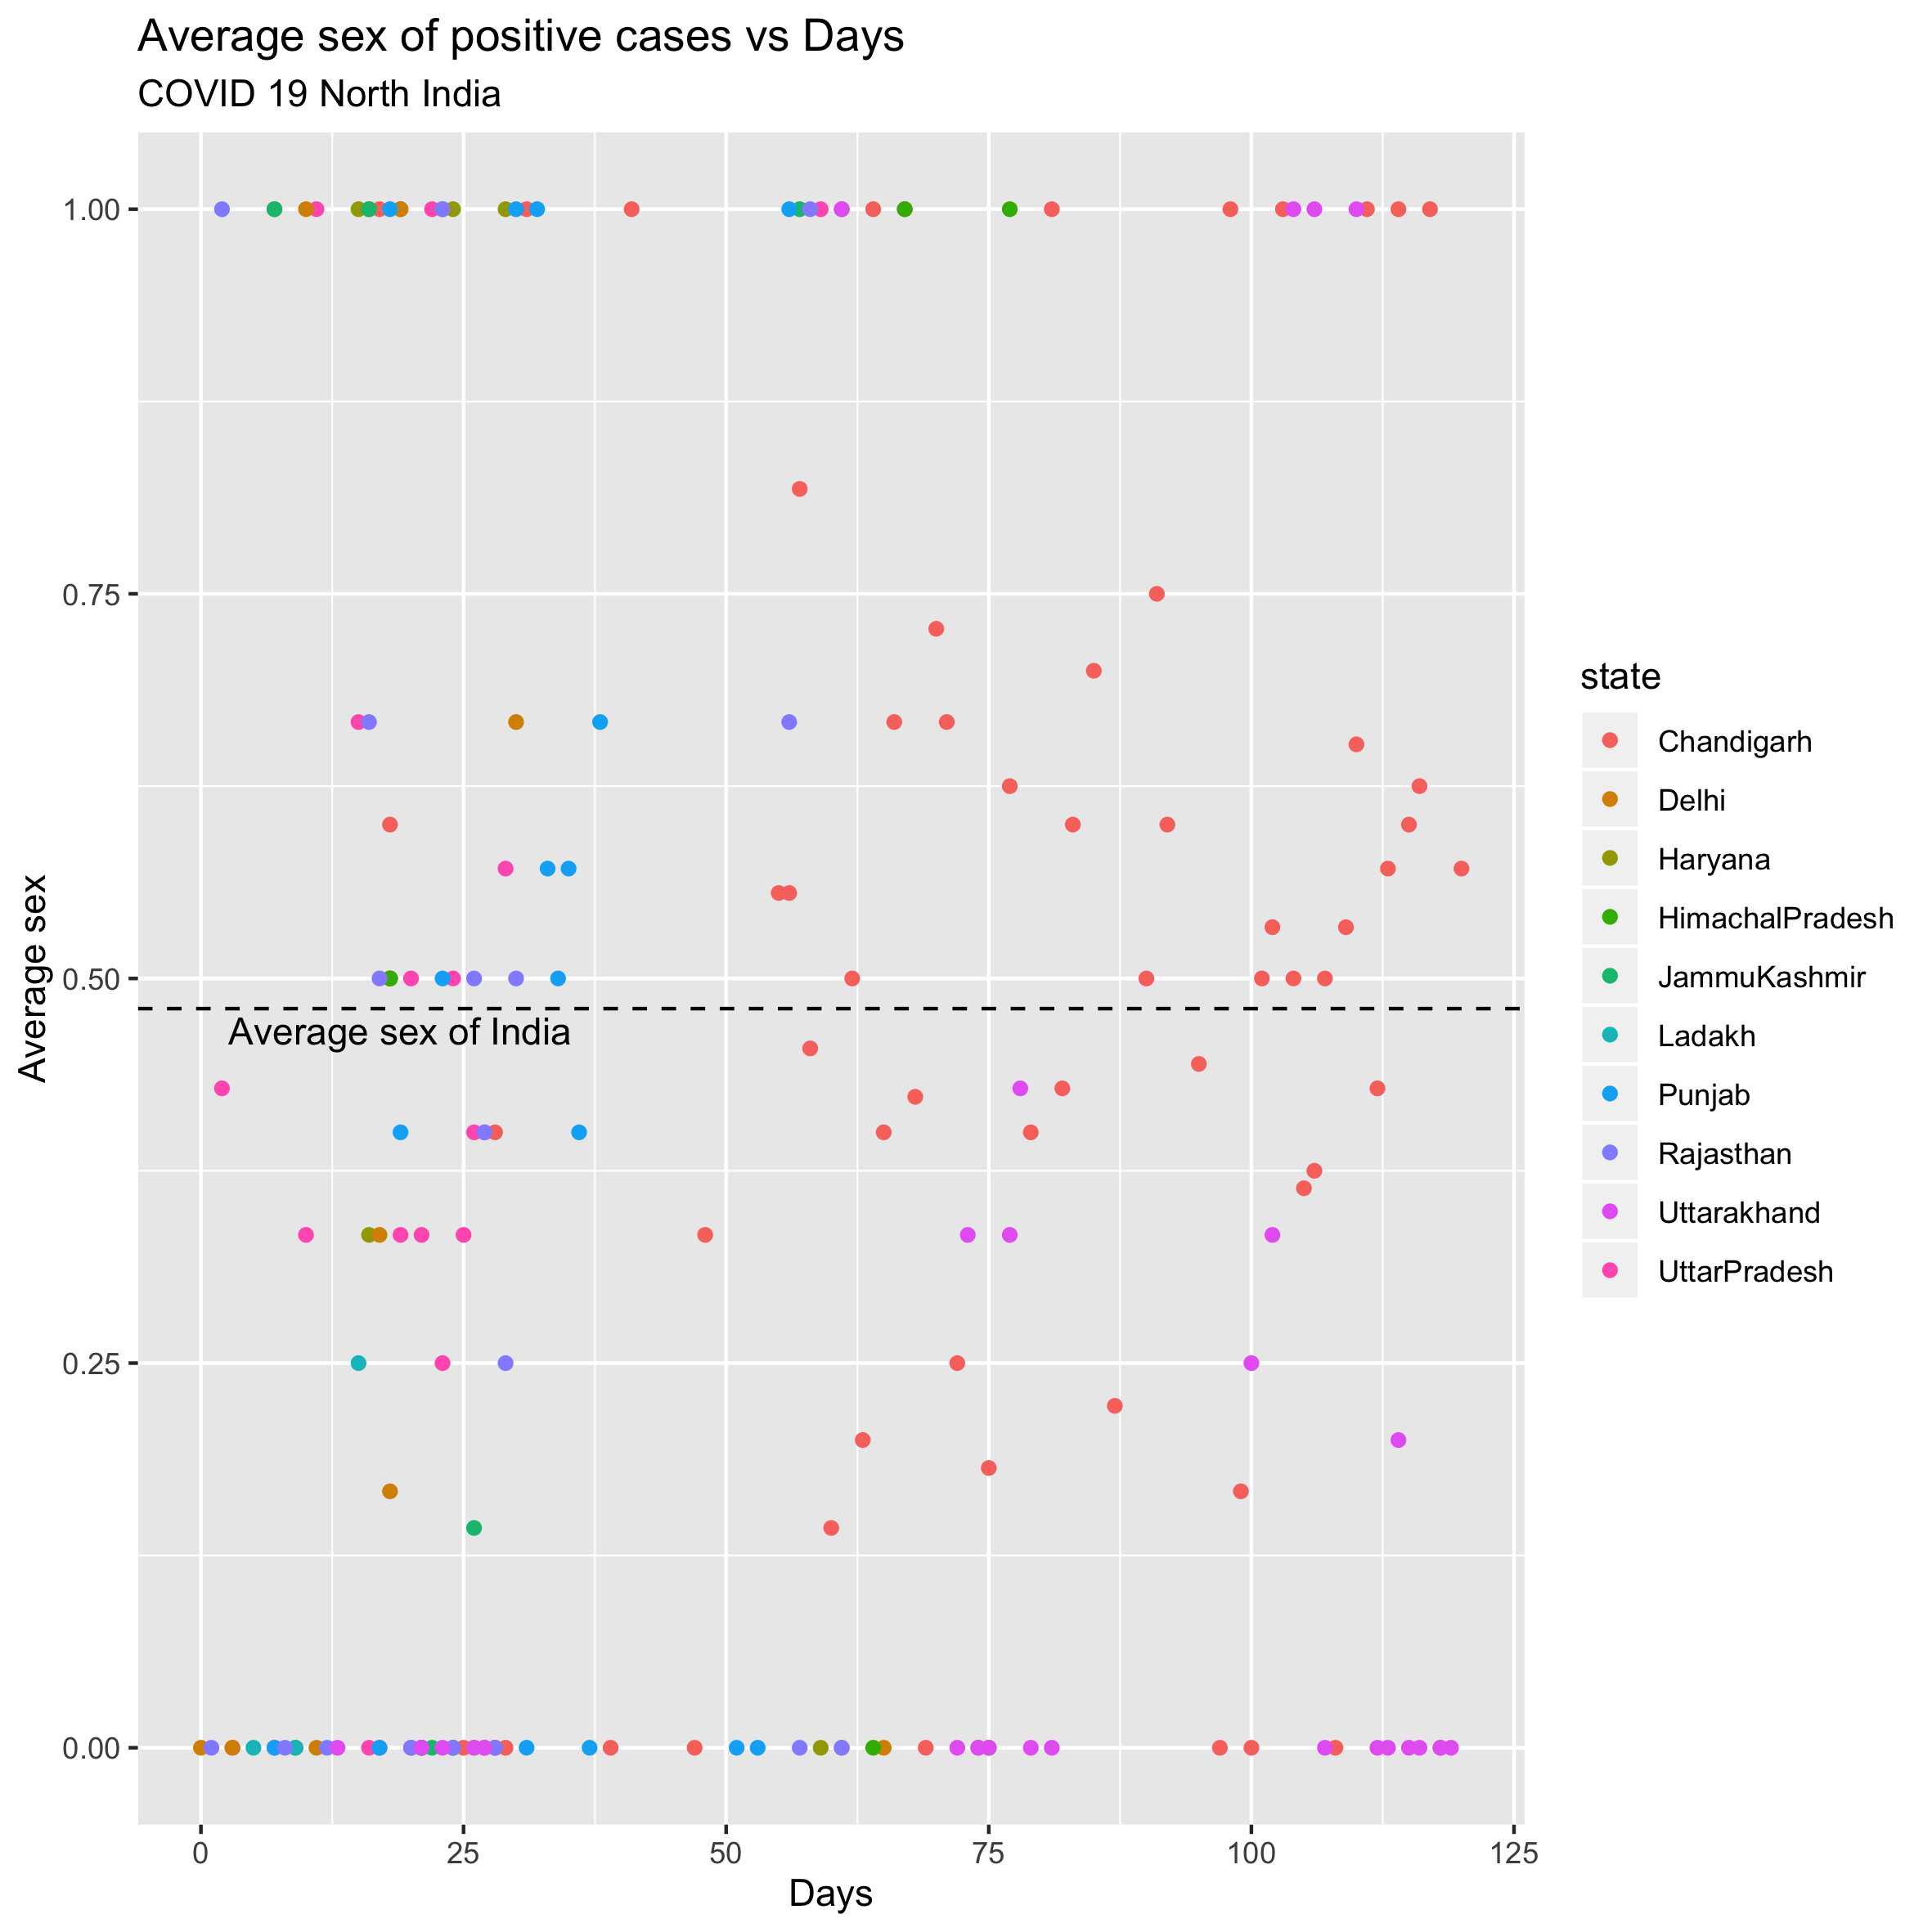
\includegraphics[scale = 0.085]{avg_sex_pos.png}
\end{frame}
%---------------------------------------------%
}

\section{\textit{A world of models of the World}}{
%---------------------------------------------%
%% SLIDE 1.4:
\begin{frame}
	\frametitle{GLM: \textit{A recap}}
	\framesubtitle{Why not just linear?}

		\begin{itemize}
		\item{Difficult modeling of \textbf{epidemiological dynamics} with (mean) linear responses;}
		\item{Nonlinear trends confirmed by visual exploratory analysis.}
		\end{itemize}
		\hfill

		\pause \center A \textbf{Linear Model} for regression: $$\text{E}[\textbf{Y}] = \textbf{X} \beta$$

		\hfill

		\pause A \textbf{Generalized Linear Model} for regression: $$\text{E}[\textbf{Y}] = \text{g}^{-1}(\textbf{X} \beta)$$
		$$ \text{Var}[\textbf{Y}] = \phi V(\text{E}[\textbf{Y}])$$
\end{frame}

\begin{frame}
	\frametitle{GLM for count data:}
	\framesubtitle{Choice of family and link function}

	\textbf{Poisson}: $$\textbf{Y} \sim \text{Poisson}(\lambda)$$
				  $$f(\textbf{Y};\lambda)=\frac{e^{-\lambda}\lambda^{\textbf{Y}}}{\textbf{Y}!}$$

	\hfill

	\textbf{Negative Binomial}: $$\textbf{Y} \sim \text{NBi}(k,\alpha)$$
				  $$f(\textbf{Y};k,\alpha)=\binom{\textbf{Y}+k-1}{k-1} \frac{\alpha^{\textbf{Y}}}{(1+\alpha)^{\textbf{Y}+k}}$$

	\hfill

	\pause \textbf{Log link function} $\rightarrow$ \textit{exponential} dynamics.


\end{frame}


\begin{frame}
	\frametitle{GLM: \textit{Predictors and Interactions} (1)}
	\framesubtitle{A matter of choosing \textbf{what} to see}

	General criterion ($\leftarrow$ \textit{NB, P, QP}):
	\begin{itemize}
		\item{Add one/some predictor(s);}
		\item{\textit{5-fold CV} \textit{cumulative MAE}} and \textit{validation cumulative MAE;}
		\item{Significance analysis on the linear coefficients.}
	\end{itemize}

		\hfill

	Starting with no \textit{lagged} component, all \textit{non-interacting} predictors:\\
	$\rightarrow$ \textbf{sequential} predictor addition always produces $r\mathcal{D}ev$ decrease;\\
	$\rightarrow$ max. \textbf{overall} significance for all parameters, for every model family.
\end{frame}
%---------------------------------------------%

\begin{frame}
	\frametitle{GLM: \textit{Predictors and Interactions} (2)}
	\framesubtitle{A matter of choosing \textbf{how} to see}

	General criterion, but also:
\begin{itemize}
	\item{Max. $2^{nd}$-order interaction;}
	\item{\textit{Non sunt multiplicanda entia sine necessitate}.}
\end{itemize}

	\hfill

	\underline{Chosen interactions} ($\leftarrow$ \textit{P, QP}):
	\begin{itemize}
		\item{\textsf{Density:Urbanization} $\rightarrow$ the \textit{vertical city} hypothesis;}
		\item{\textsf{Males:Urbanization} $\rightarrow$ the \textit{male migration} hypothesis in India}.
	\end{itemize}

	\hfill

	The case of \textsf{Urbanization}: \textit{significance absorption} and \textit{predictive accuracy}.

\end{frame}
%---------------------------------------------%

%---------------------------------------------%

\begin{frame}
	\frametitle{GLM: \textit{Predictors and Interactions} (3)}
	\framesubtitle{A matter of choosing \textbf{when} to see}

	Introduction of \textit{lagged} components:
	\begin{itemize}
		\item{Justified theoretically by phenomenon structure;}
		\item{\textit{But will they really work?}}
	\end{itemize}

	\hfill

	General criterion ($\leftarrow$ \textit{NB, P, QP}):
	\begin{itemize}
		\item{Add one/some \textit{lagged} component(s);}
		\item{\textit{Validation cumulative MAE};}
		\item{Significance analysis on the \textit{lagged}-component coefficients.}
	\end{itemize}

	\hfill

	\underline{Results}:\\
	$\rightarrow$ No \textit{cross-regressive lagged} predictor is useful;\\
	$\rightarrow$ Autoregressing on response (lagged at $10$ days) helps P/QP.

\end{frame}

\begin{frame}
	\frametitle{GLM: \textit{Predictors and Interactions} (4)}
	\framesubtitle{A picture is worth a thousand words: the final model (QP)}

	\begin{center}
		\center 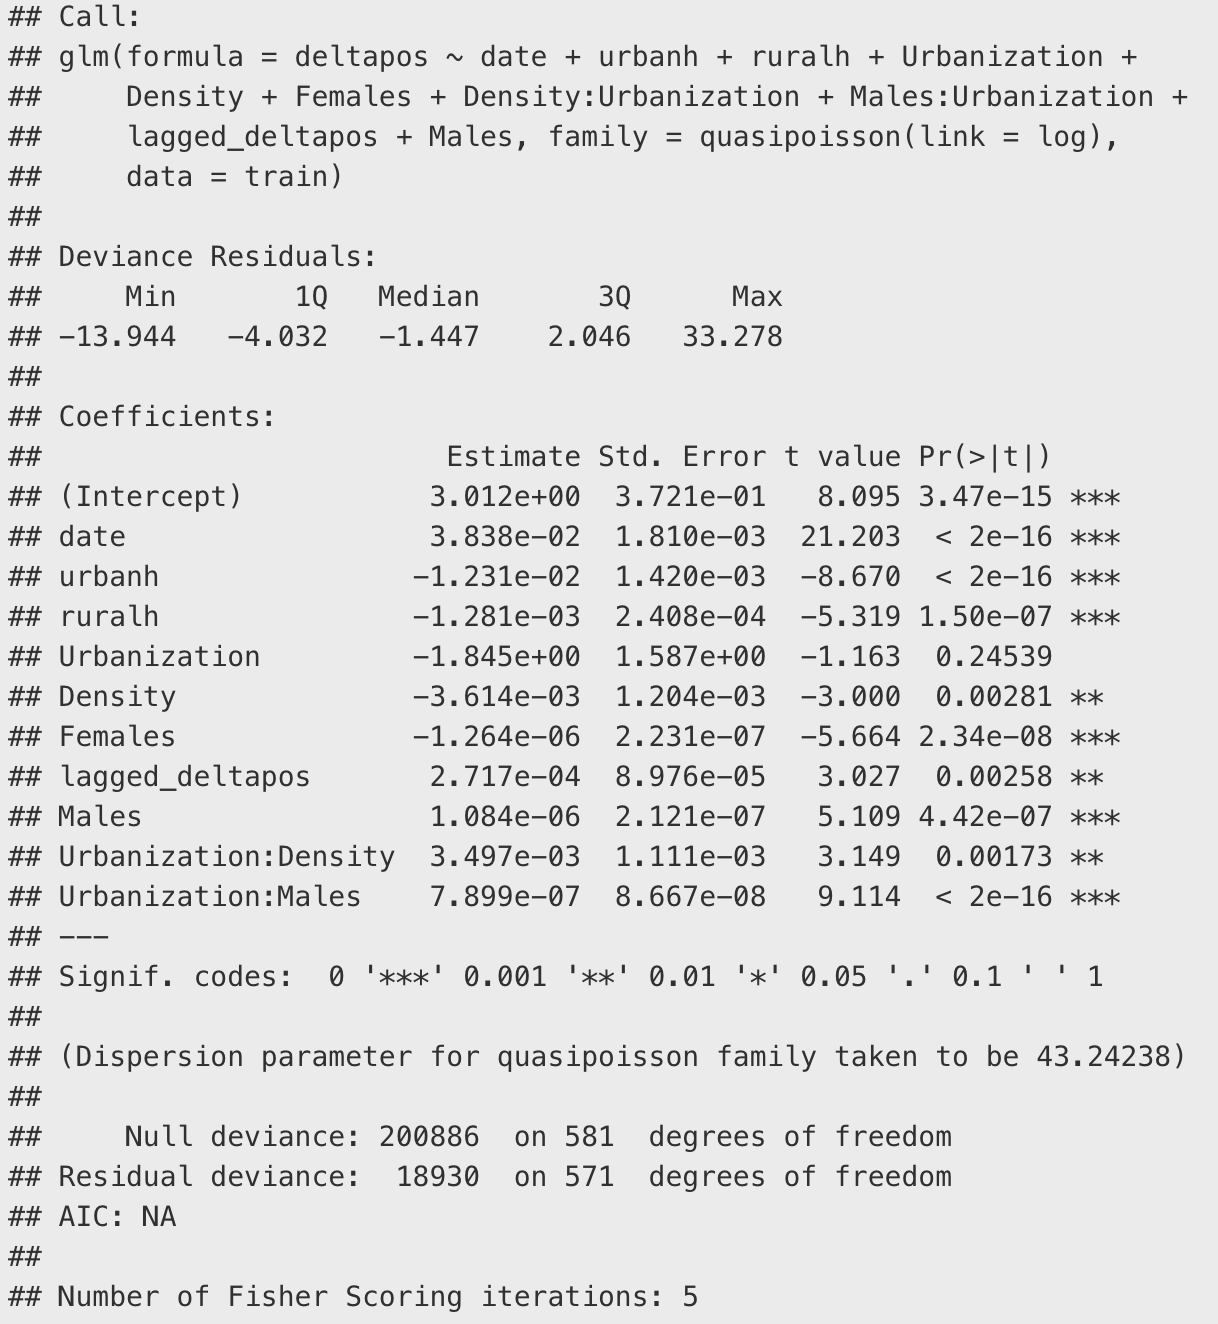
\includegraphics[scale = 0.3]{summary_qpoisson.png}
	\end{center}


\end{frame}
%---------------------------------------------%
%% SLIDE 1.5:
\begin{frame}
	\frametitle{GLM: \textit{Predictors and Interactions} (5)}
	\framesubtitle{A picture is worth a thousand words: the MLE model (P)}
		\center 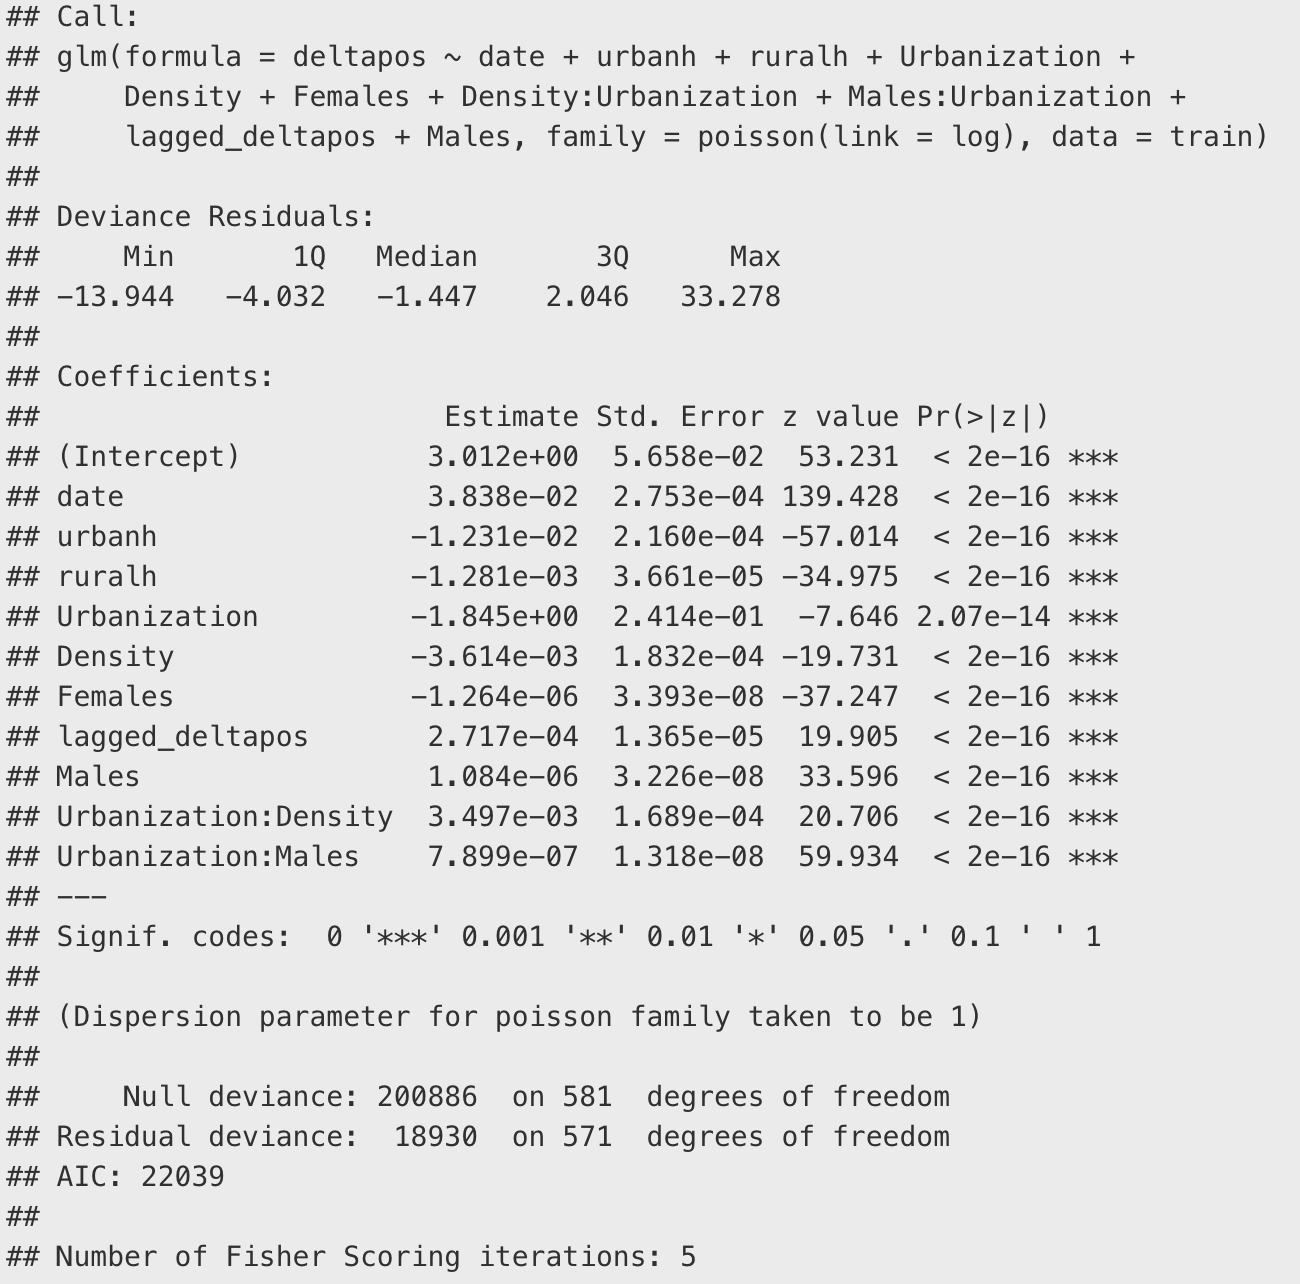
\includegraphics[scale = 0.3]{summary_poisson.png}
	\end{frame}
%---------------------------------------------%
%% SLIDE 1.5.1:
\begin{frame}
	\frametitle{GLM: \textit{Predictors and Interactions} (6)}
	\framesubtitle{A picture is worth a thousand words: the case of \textsf{Urbanization}}
	\center 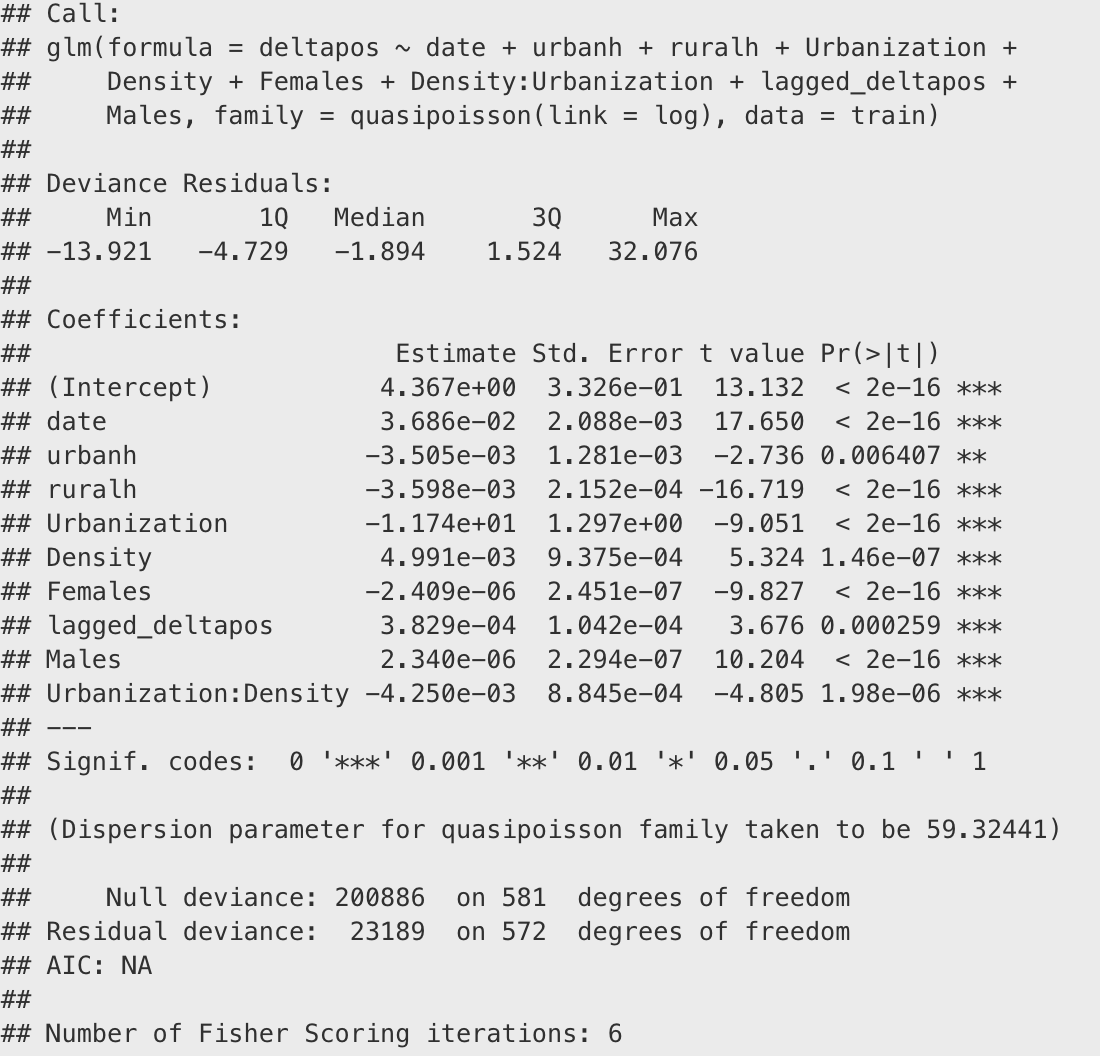
\includegraphics[scale = 0.38]{summary_qpoisson_urb.png}
\end{frame}
%---------------------------------------------%
%% SLIDE 1.5.2:
\begin{frame}[t]

	\frametitle{GLM: \textit{Determining prediction intervals}}
	\framesubtitle{A \textit{bootstrap} way }
	Generally, prediction intervals for GLMs are not easily computable...
	\\~\\
	Bootsrap-based solution:
	\begin{itemize}
		\item Fit the GLM, and collect the regression statistics $\hat{\beta}$ and $\text{Cov}(\hat{\beta})$:
		\item Simulate M draws of $\hat{\beta}^{*} \sim N(\hat{\beta}, \hat{\mathrm{Cov}}(\hat{\beta}))$;
		\item Simulate $y^*| x$ from response $g^{-1}(x \hat{\beta}^{*})$ and a variance determined by the response distribution;
		\item Determine the $\alpha/2$ and $1-\alpha/2$ empirical quantiles of the simulated response $y^*|x$ for each x.
	\end{itemize}
	~\\
	Possibility to reparametrize a Quasipoisson model into a Negative Binomial using $\mathrm{QP}(\mu, \theta) = \mathrm{NegBin}(\mu, \theta = \frac{\mu}{\phi - 1}).$
\end{frame}
%---------------------------------------------%

%---------------------------------------------%
%% SLIDE 1.6:
\begin{frame}[t]
	\frametitle{MARS: \textit{A recap} (1)}
	\framesubtitle{A \textit{nice} piecewise linear model (Friedman, 1991)}

	Multivariate Adaptive Regression Splines (MARS) model response as a weighted sum of basis functions
	$$ \widehat{f}(x) = \sum_{i=1}^k c_i B_i(x). $$


	The basis functions $B_i(x)$ takes one of the three forms:

	\begin{itemize}
		\item a constant 1;
		\item hinge function:  $\max(0, x - k)$ or $\max(0, k - x), ~ k: \ \text{``knot''}$;
		\item product of two or more hinge functions.
	\end{itemize}


\end{frame}

\begin{frame}[t]
	\frametitle{MARS: \textit{A recap} (2)}
	\framesubtitle{The model building process}
	Two-stage approach:
	\begin{itemize}
		\item \textit{Forward pass}: incrementally adding basis function that gives maximum reduction in sum-of-squares residual error;
		\item \textit{Backward pass}: delete least effective term using GCV criterion.
	\end{itemize}

	~\\ \textit{HP-tuning}: \\
	$\rightarrow$ grid-search, 5-fold CV minimizing the cumulative MAE:
	\begin{itemize}
		\item degree: 1 by 1, from 1.
	\end{itemize}

\end{frame}

\begin{frame}[t]
	\frametitle{MARS: \textit{A recap} (3)}
	\framesubtitle{\textit{Why that?}}
	A non parametric regression method.
	\\~\\
	Pros:
	\begin{itemize}
		\item More flexible than linear models;
		\item Simple to understand and interpret compared to other ML-based solutions;
		\item Automated modelling of interactions.
	\end{itemize}


	Cons:
	\begin{itemize}
		\item The resulting fitted function is not smooth (not differentiable along predictors);
		\item \textit{Greedy optimization vs. global optimization}.
	\end{itemize}
\end{frame}

\begin{frame}
	\frametitle{MARS: \textit{Predictors and Interactions}}
	\framesubtitle{A summary}
	\center 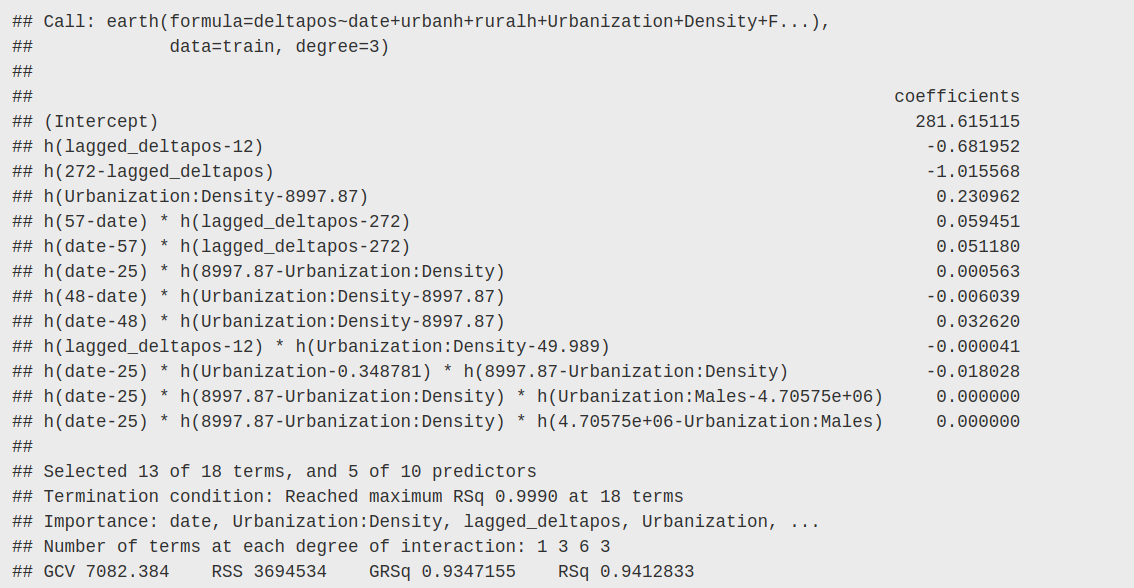
\includegraphics[scale = 0.26]{summary_mars.png}
\end{frame}

\begin{frame}
	\frametitle{MARS: \textit{Determining prediction intervals}}
	\framesubtitle{Residual model (Stephen Milborrow, 2019)}

	We do the following:

	\begin{itemize}
		\item Estimate the mean absolute error at each point using a \textit{residual model};
		\item Assuming normality, re-scale the error to an estimated standard deviation: $sd \simeq \sqrt{\frac{\pi}{2}} \text{E}[{|\epsilon|}]$;
		\item Convert the standard deviation to an estimated prediction interval for a given level $\alpha$:
		$$ [\hat{Y}-z_{\alpha/2}sd, \hat{Y}+z_{\alpha/2}sd]. $$
	\end{itemize}

\end{frame}
%---------------------------------------------%

\begin{frame}
	\frametitle{RF: \textit{A recap} (1)}
	\framesubtitle{Harnessing the \textit{wisdom of the crowd}}

	Based on the \textbf{decision tree} (regression) model and learning algorithm.

	\hfill

	Enhancements:
	\begin{itemize}
		\item{\textbf{Bootstrap} sampling on \textit{training set};}
		\item{\textbf{Random} feature selection;}
		\item{\textbf{Ensembling} of aggregates}.
	\end{itemize}

	\hfill

	\textit{HP}-tuning:\\
	$\rightarrow$ grid-search, \textit{5-fold CV} test \textit{cumulative MAE}:
	\begin{itemize}
		\item{\textsf{mtry}: $1$ by $1$, from $1$ $\rightarrow$ 5;}
		\item{\textsf{num.trees}: $10$ by $10$, from $500$ $\rightarrow$ 850.}
	\end{itemize}


\end{frame}


\begin{frame}
	\frametitle{RF: \textit{A recap} (2)}
	\framesubtitle{\textit{Why that?}}

	On the opposite side of the spectrum w.r.t. GLMs.

	\hfill

	Pros:
	\begin{itemize}
		\item{Typical \textit{fire and forget} \textbf{ML}-based solution;}
		\item{Often requires minimal \textit{HP-tuning};}
		\item{\textit{Automated} modeling of \textbf{interactions}.}
	\end{itemize}

	\hfill

	Cons:
	\begin{itemize}
		\item{Only averaged or modal \textbf{stepwise} regression capability;}
		\item{Difficult to interpret;}
		\item{May sometimes overfit or fit noise;}
		\item{\textbf{Non-deterministic} behavior and seed-dependence.}
	\end{itemize}

\end{frame}


\begin{frame}
	\frametitle{RF: \textit{Determining prediction intervals}}
	\framesubtitle{\textit{Always beware of absolute certainty!} (Zhang et al., 2019)}

	A well-acknowledged problem for \textit{tree-based} models...

	\hfill

	...and a new proposal:
	$$
	\left[ { \hat{Y} + D_{\left[ { n, \alpha/2 } \right]}, \hat{Y} + D_{\left[ { n, 1-\alpha/2 } \right]} } \right]
	$$

	\hfill

	\begin{itemize}
		\item{Uses the \textit{empirical quantile distribution} of \textbf{OOB prediction} errors;}
		\item{Well-grounded from the \textbf{asymptotic convergence} p.o.v.;}
		\item{Easy to compute, often partially pre-computed \textit{for free};}
		\item{\textsf{R} implementation already available!}
	\end{itemize}
\end{frame}


}

\section{\textit{Results}}{
	%---------------------------------------------%
	%% SLIDE 1.8:
	\begin{frame}
		\frametitle{QuasiPoisson model}
		\framesubtitle{Predictions and Prediction Intervals}
		\center 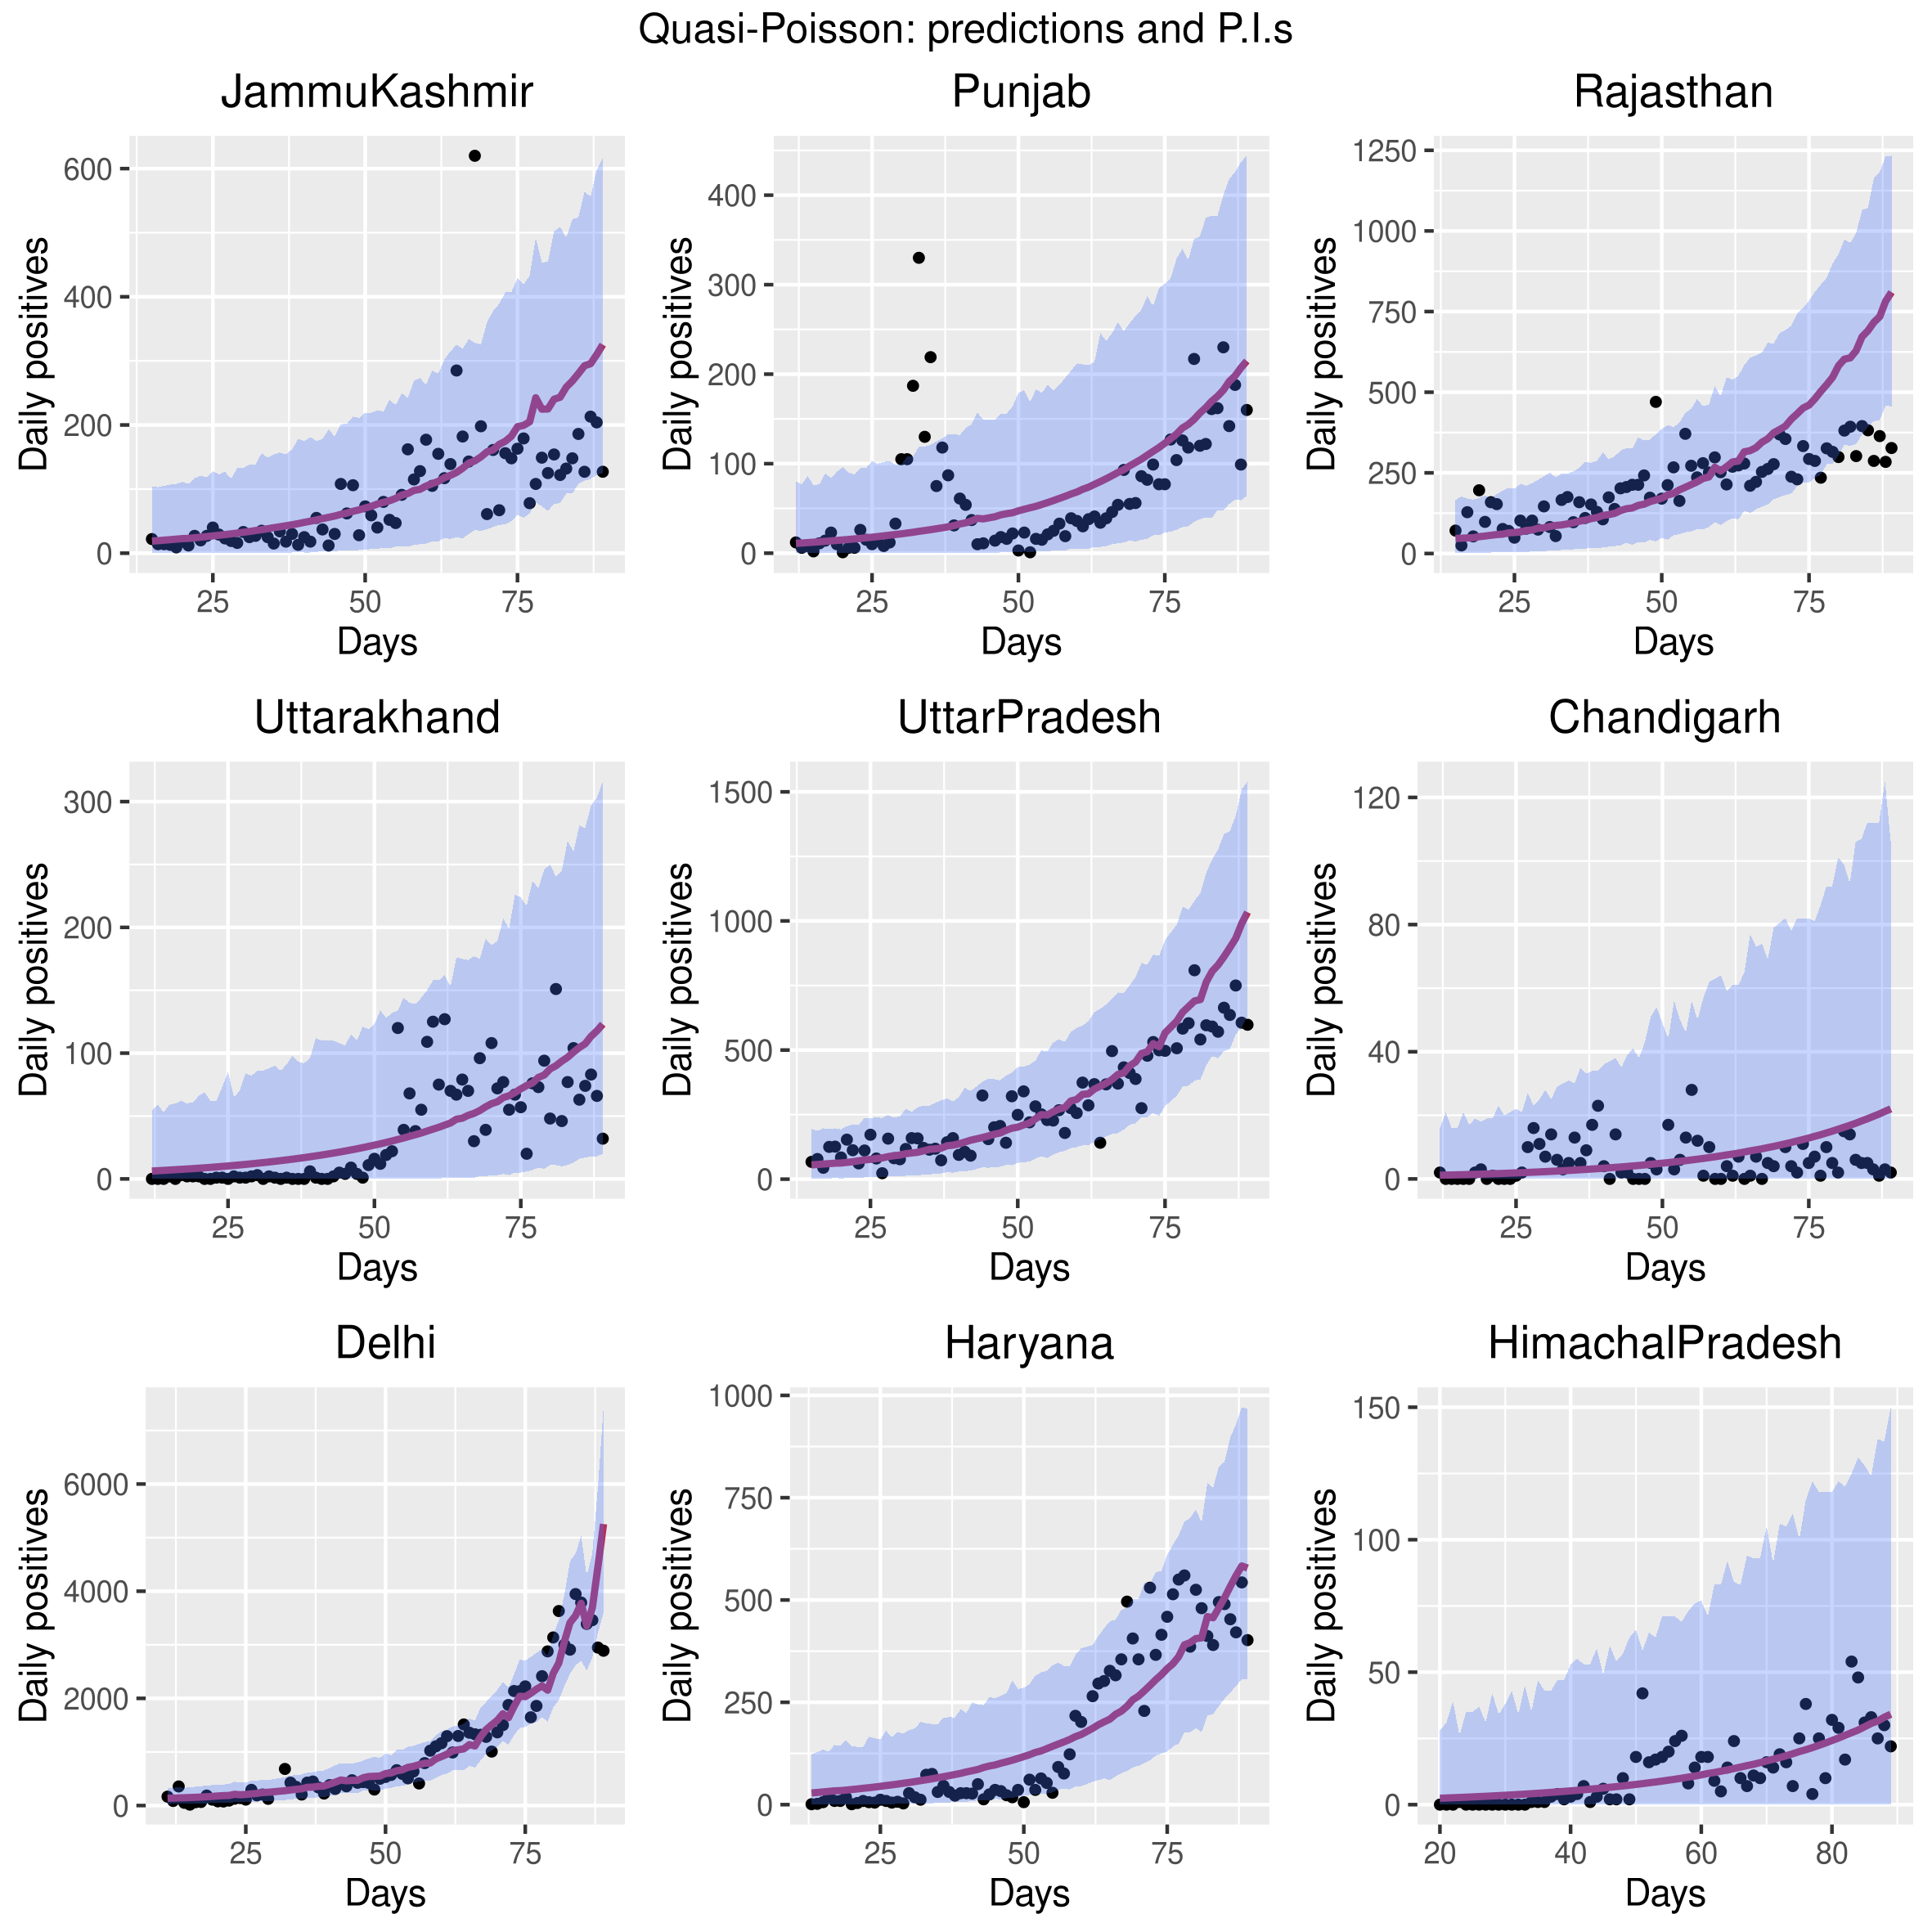
\includegraphics[scale = 0.37]{qp_ppi.png}
	\end{frame}
	%---------------------------------------------%
	%% SLIDE 1.9:
	\begin{frame}
		\frametitle{MARS model}
		\framesubtitle{Predictions and Prediction Intervals}
		\center 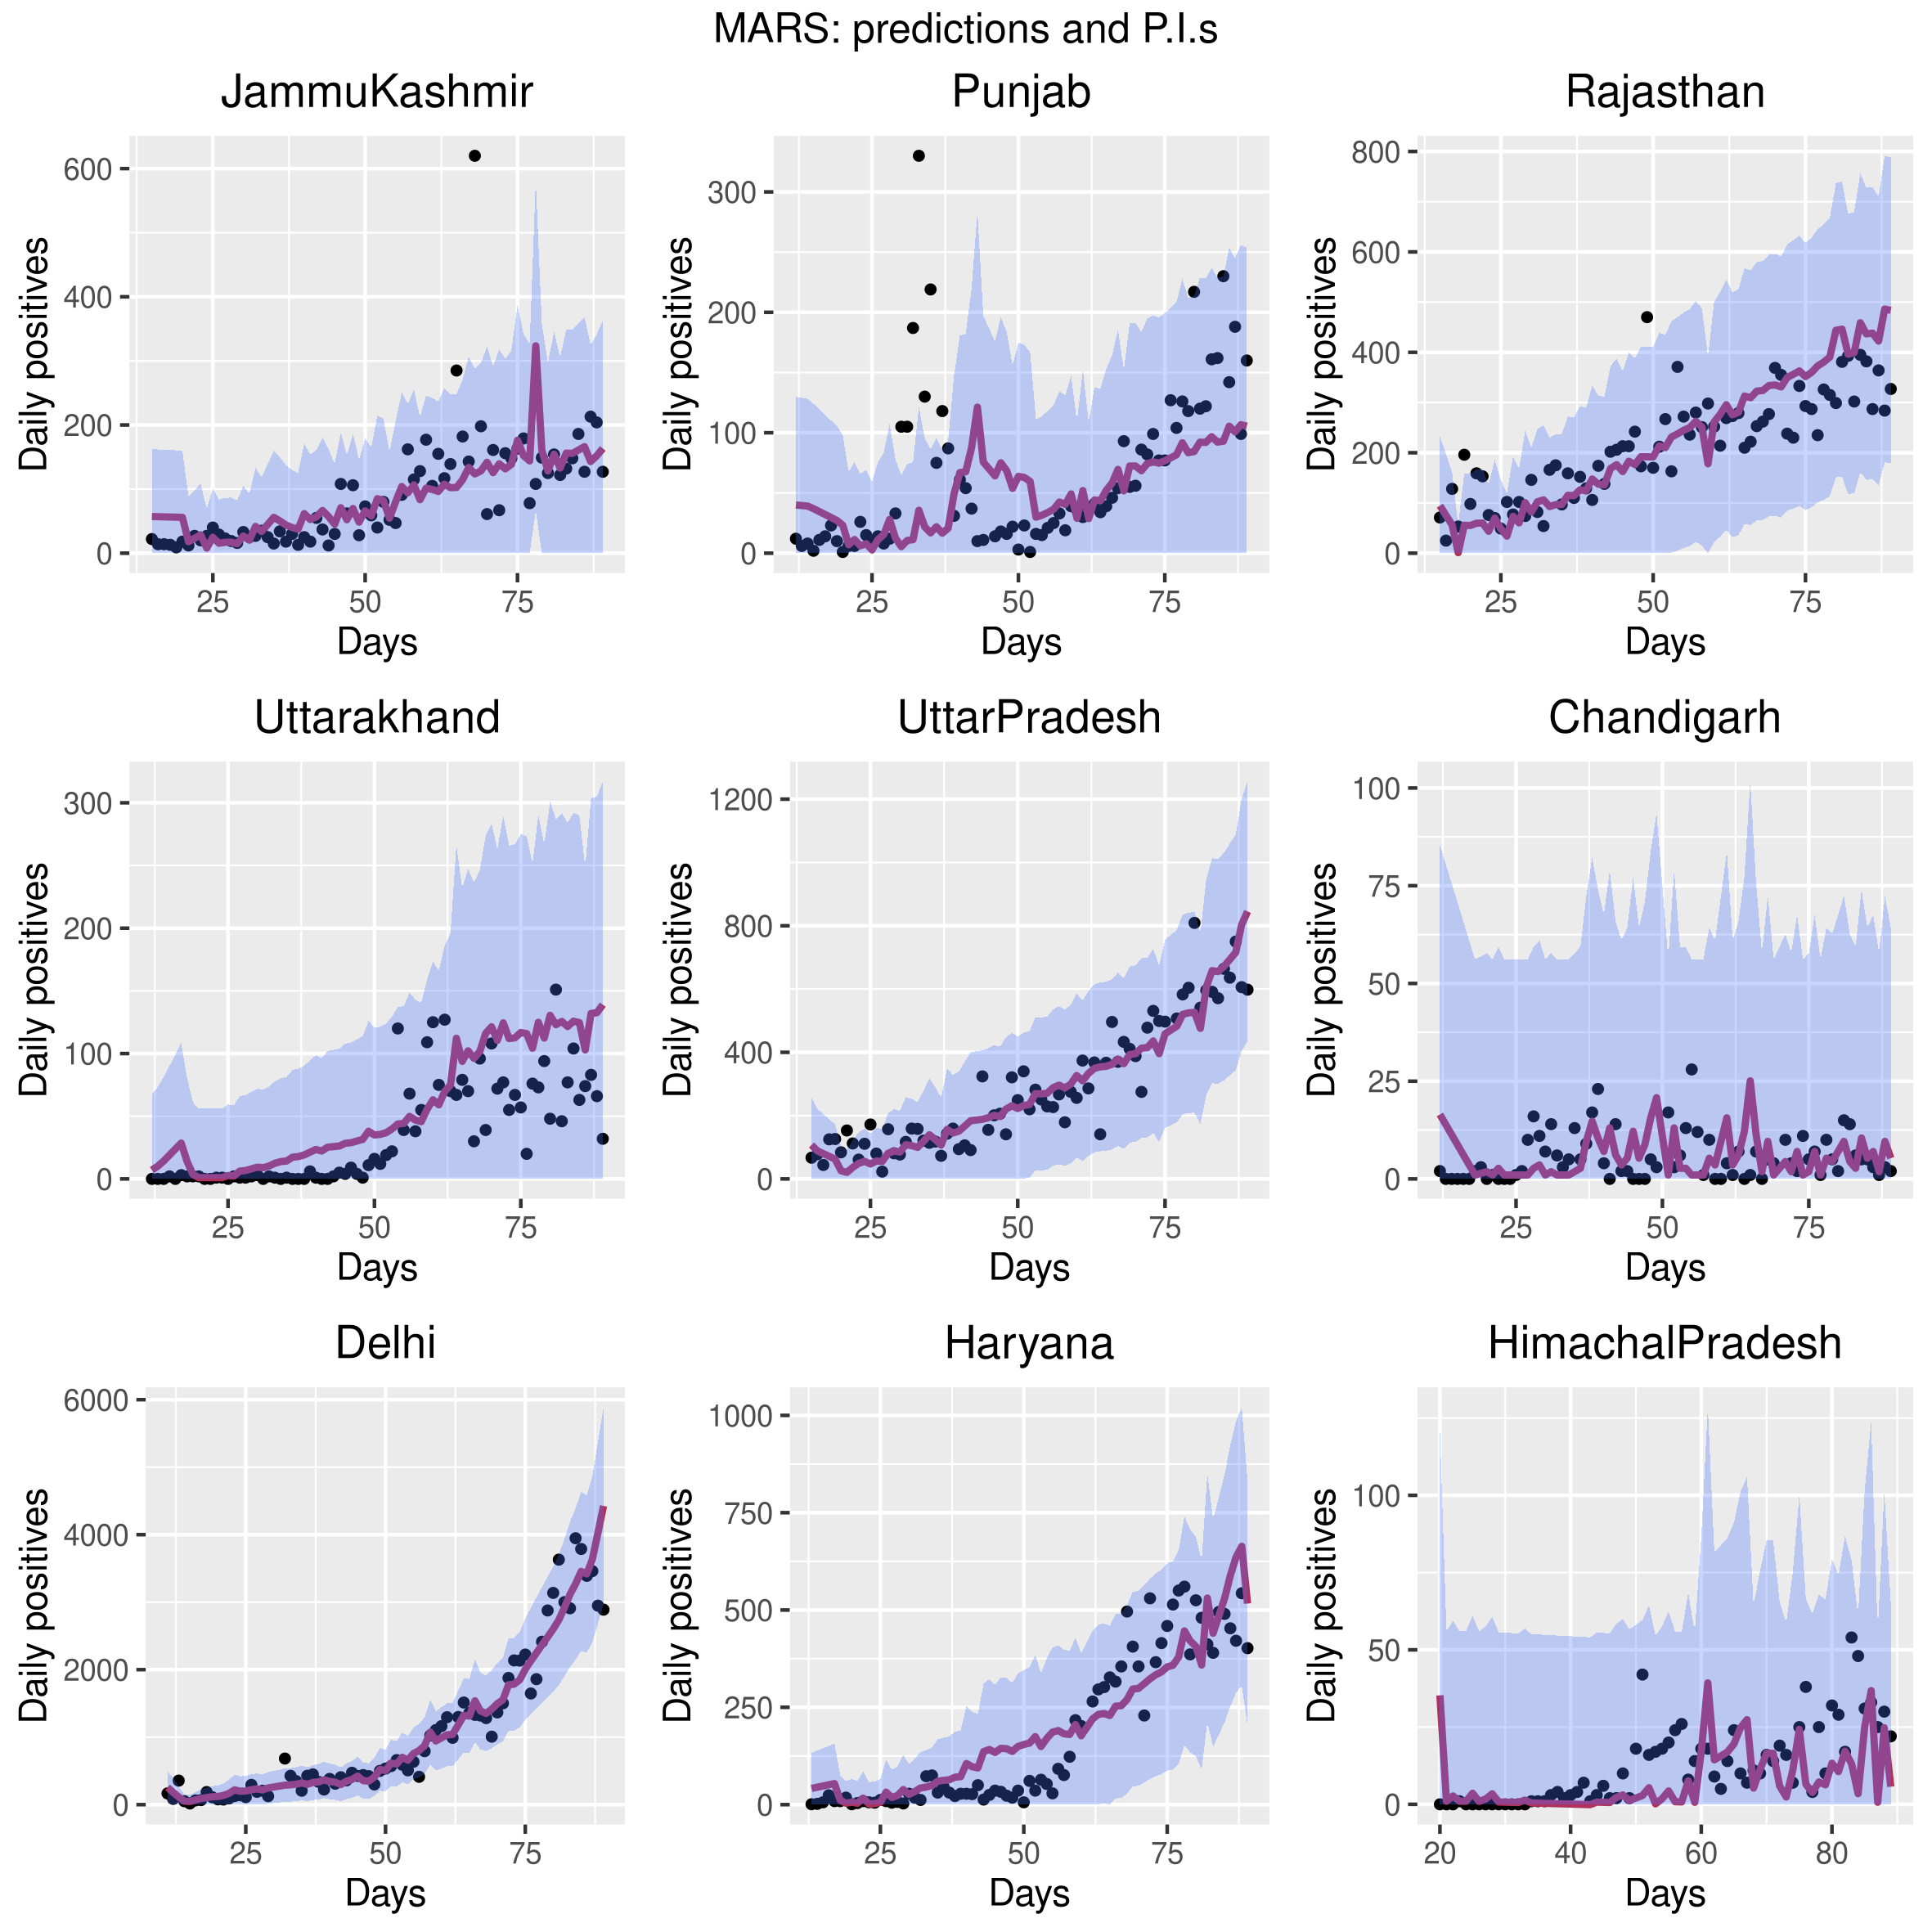
\includegraphics[scale = 0.37]{mars_ppi.png}
	\end{frame}
	%---------------------------------------------%
	%% SLIDE 1.10:
	\begin{frame}
		\frametitle{Random Forest model}
		\framesubtitle{Predictions and Prediction Intervals}
		\center 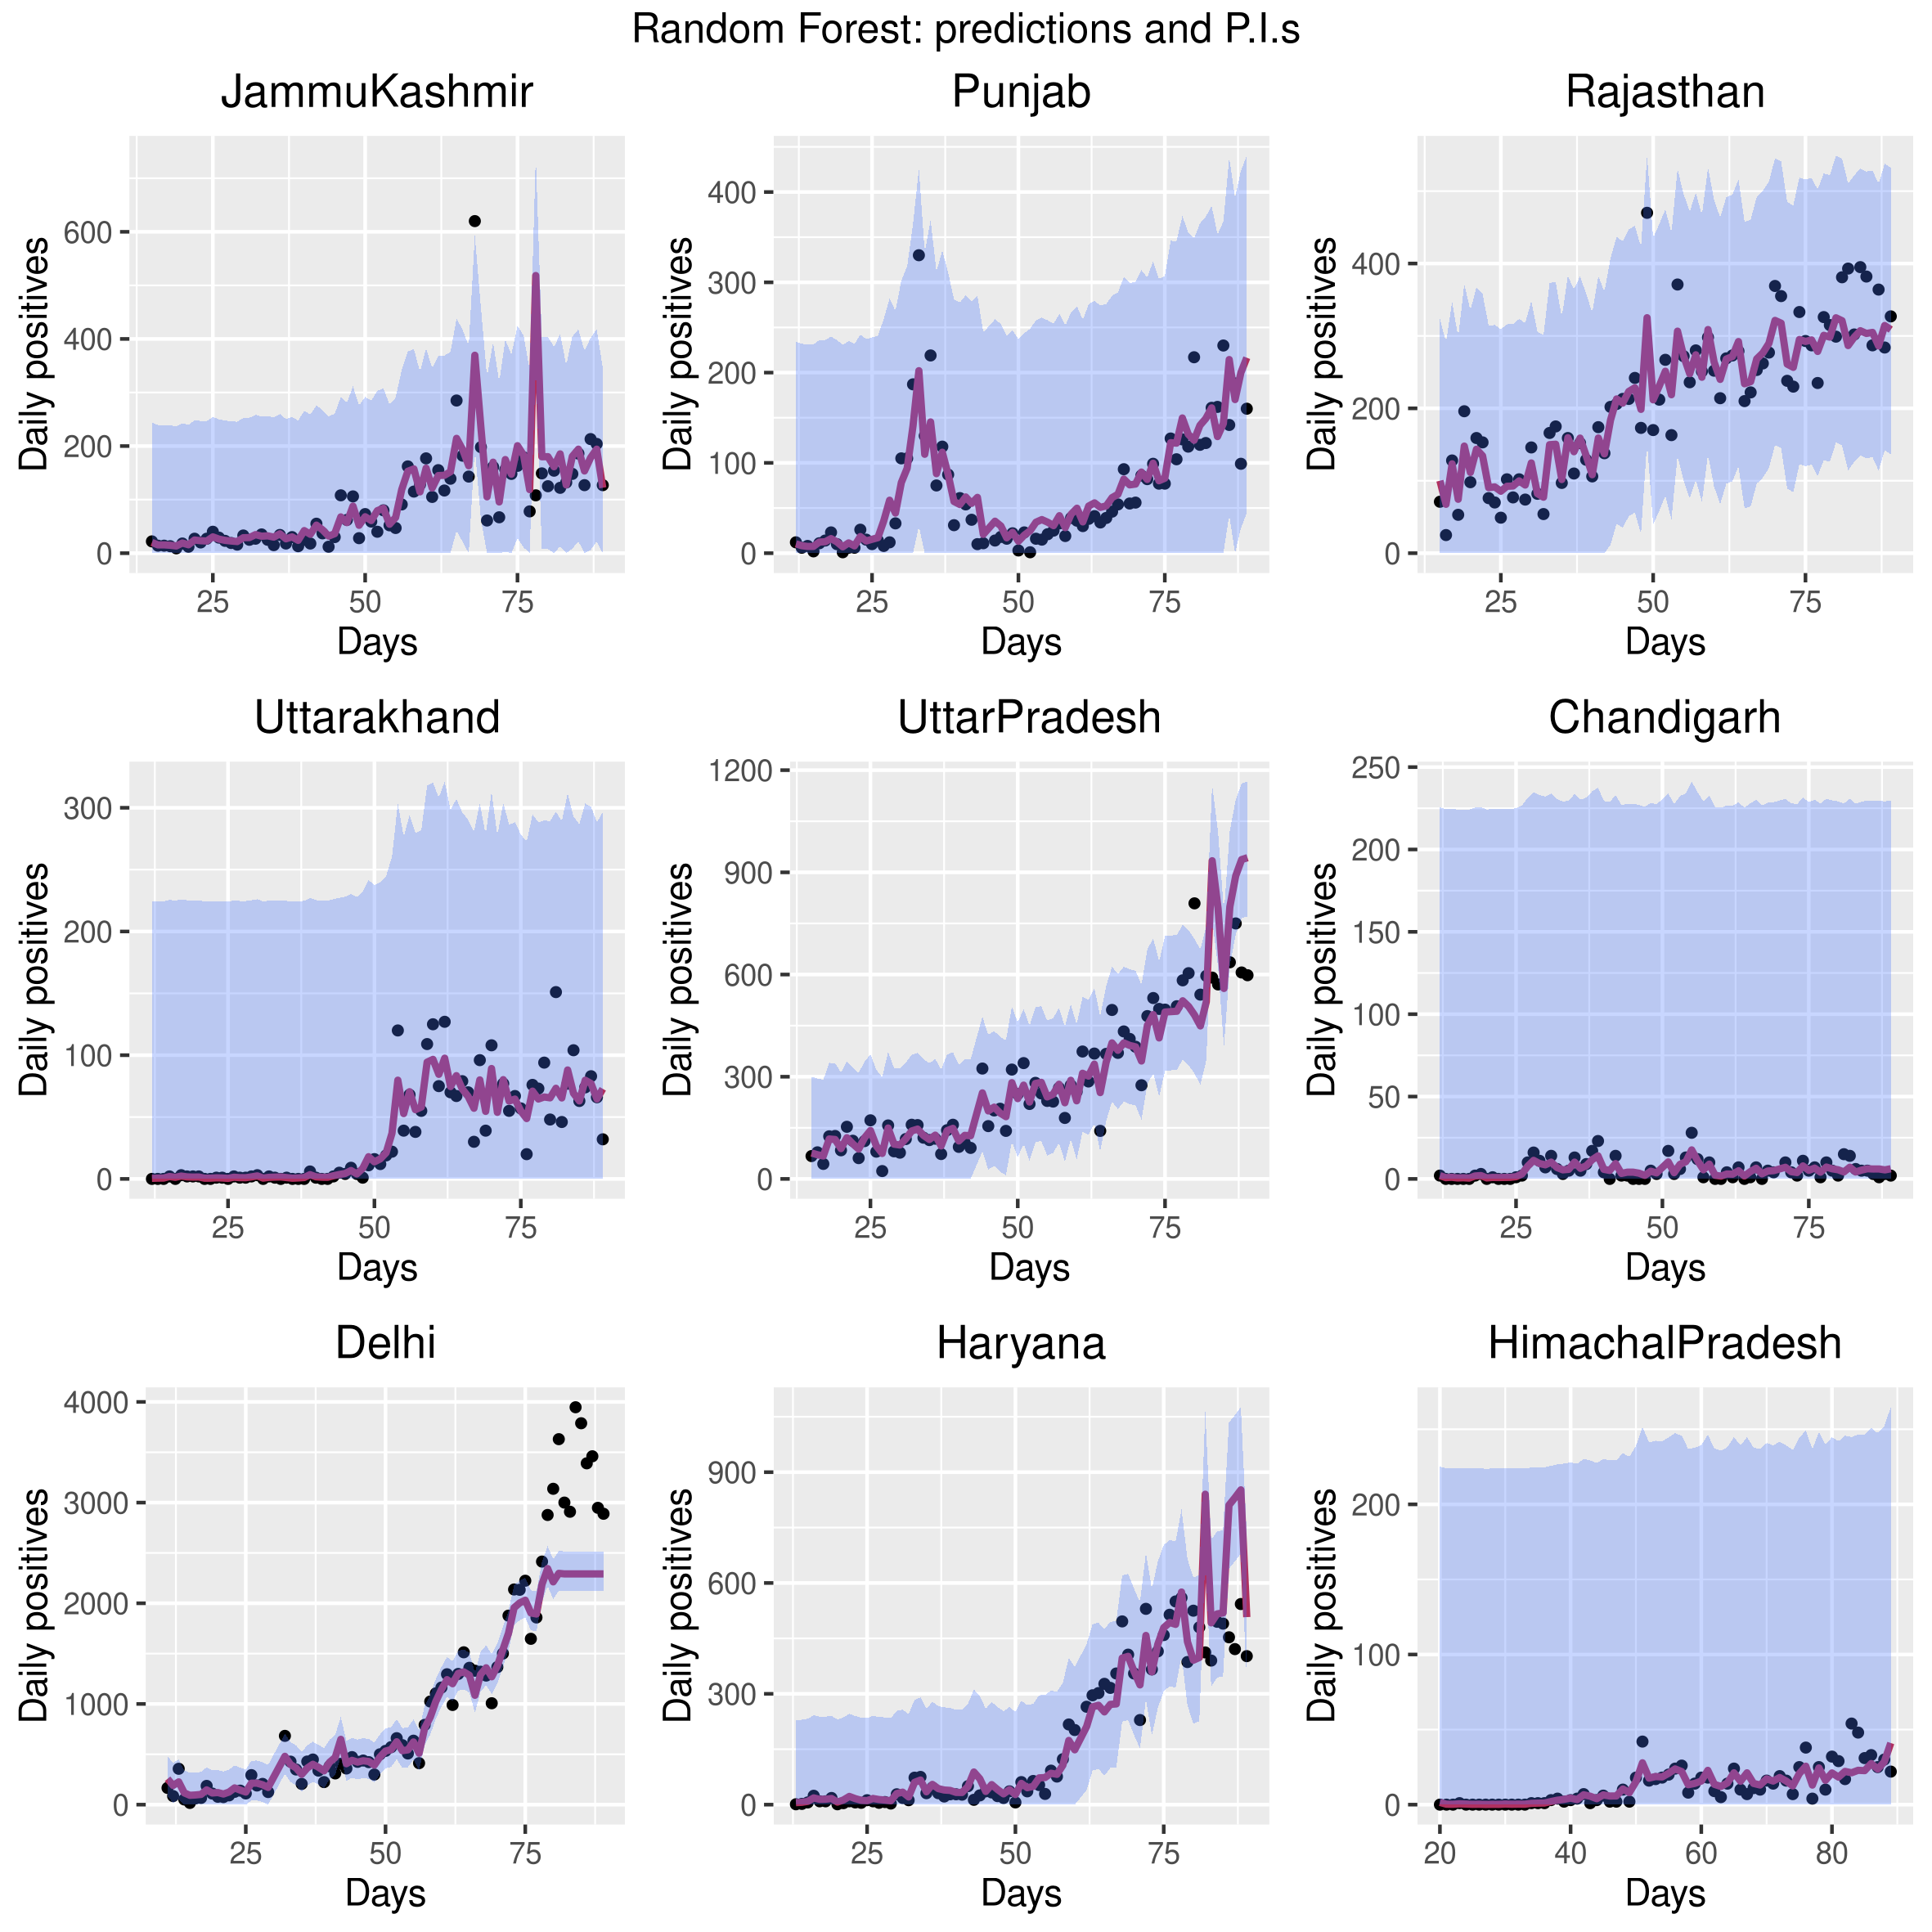
\includegraphics[scale = 0.37]{rf_ppi.png}
	\end{frame}
	%-----------------------------------------------%
	%% SLIDE 1.11:
	\begin{frame}
		\frametitle{Accuracy measure: RMSE}
		\framesubtitle{Accuracy is not everything}
		\center 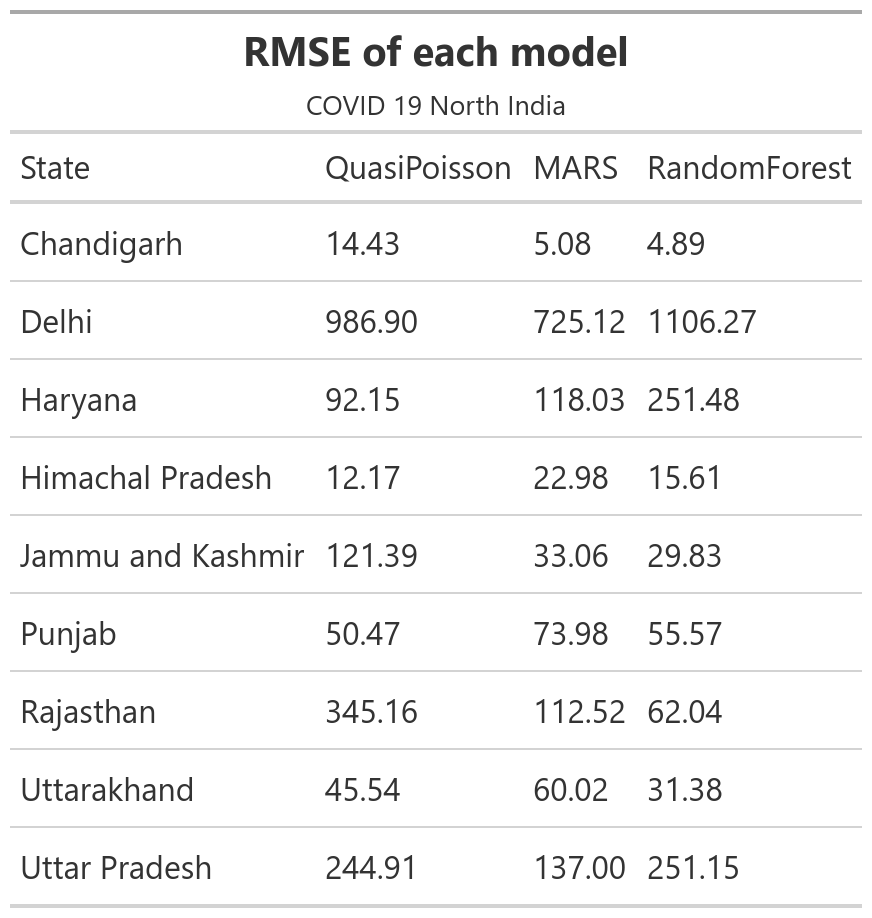
\includegraphics[scale = 0.2]{acc_tab.png}
	\end{frame}
}

\section{\textit{Conclusions}}{
	%---------------------------------------------%
	%% SLIDE 1.12:
	\begin{frame}
		\frametitle{Final remarks}
		\framesubtitle{\textit{ML vs. Stats} doesn't belong to the real world}
		\hfill \break
		Parametric model:
		\begin{itemize}
			\item{QuasiPoisson model correctly captures the pandemic trend;}
			\item{On average, it has a higher RMSE than non parametric models, partly due to noisy data.}
		\end{itemize}
		\hfill \break
		Non parametric models:
		\begin{itemize}
			\item{Sometimes MARS and Random Forest favor local over global trends;}
			\item{Random Forest predictions are unstable.}
		\end{itemize}
		\hfill \break
		Trade-off between analyst's \textit{cognitive burden} and model ability to grasp deep inter-connections about reality.

	\end{frame}

}

%% THANKS!
\begin{frame}
	\frametitle{Greetings}
		\center Thank you for your attention!
		\center 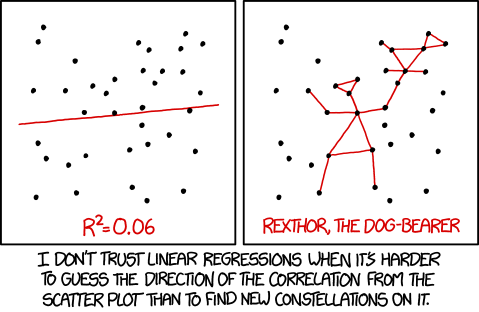
\includegraphics[scale = 0.5]{rexthor.png}
		\center [\url{https://github.com/emaballarin/northindia-covid-smds}]
\end{frame}

%-----------------------------------------------%
\end{document}
